\chapter{Integrated Sensing and Two-Tier Task Offloading via NOMA: An Energy-Minimization Design}
\label{chap5_twc2}

\section{Introduction} 

The rapid developments of next-generation communication technologies have yielded tremendous revolutions in emerging immersive services such as Metaverse, smart healthcare, and autonomous driving, which necessitate diverse quality of services including high-precision sensing, ultra-reliable communications, and low-latency computing \cite{twc2.liu2022integrated}. Mobile edge computing (MEC), which allows edge computing users with limited processing capabilities to offload tasks to nearby edge servers, has been considered as an effective solution for reducing computing latency \cite{twc2.mao2017survey,intro.8030322,intro.7879258}. Concurrently, integrated sensing and communication (ISAC) provides a key paradigm for achieving simultaneous high-throughput transmission and high-precision sensing within limited spectrum resources \cite{twc2.9393464,intro.11111722,intro.10217169,intro.10833779}. Consequently, the convergence of these technologies into integrated sensing, communication, and computing (ISCC) networks is expected to play a crucial role in future wireless networks, offering enhanced collaboration capabilities and efficient resource utilization. In particular, realizing the full potential of ISCC requires careful design of interference mitigation and resource allocation strategies.

Non-orthogonal multiple access (NOMA), which allows multiple users to be served simultaneously on the same resource block, has been considered as a spectrum-efficient approach to enable massive connectivity in next-generation wireless networks \cite{intro.8886467}. By using superposition coding (SC) at the transmitter side and further using successive interference cancellation (SIC) at the receiver side, NOMA can mitigate users' co-channel interference, which has attracted a lot of research interests in exploiting NOMA for various wireless services \cite{twc2.10255731,twc2.9507329,intro.9133094,intro.9154358,intro.11106811}. In particular, NOMA has been regarded as a promising solution for alleviating severe inter-functionalities interference in ISCC systems under massive connectivity.

With the exponential growth of network traffic and environmental sensing data, a single-tier edge computing framework relying solely on local edge servers cannot meet the escalating demands of ISCC networks. Leveraging multi-tier cooperative edge computing, where edge servers and cloudlet servers are jointly utilized for task processing, enables an efficient and balanced utilization of computing resources across different tiers, thereby avoiding the severe processing delay due to the potential congestion caused by overloading.
In this chapter, we investigate a NOMA-assisted integrated sensing and two-tier task offloading (ISTTO) framework, in which an ISCC access point (AP) provides task offloading services for a group of edge computing users via NOMA while performing the radar sensing towards a target in both tiers. The signals in the two tiers are illustrated as follows.
In Tier-I, the AP transmits a sensing signal to sense the target. Meanwhile, the AP receives both the sensing echo and all edge computing users' offloading signals. In Tier-II, the AP transmits the ISAC signal (including the dedicated sensing signal and the offloading signals), which is used to offload the workloads to a group of cloudlet servers and perform the radar sensing simultaneously. Our framework poses two important challenges as follows.
First, the sensing and offloading signals interfere with each other in Tier-I, while only the dedicated sensing signal interferes to the offloading signals in Tier-II. 
It is crucial to design different NOMA mechanisms for alleviating different inter-functionalities interferences and thus improve the performances of both sensing and offloading. 
Second, in the two-tier framework, there exists a tradeoff between the sensing accuracy and the computational offloading latency by properly tuning the durations of Tier-I and Tier-II.
Specifically, the longer durations of Tier-I and Tier-II allow for a larger amount of sensing estimation information, and consequently yield an improved estimation of the target. However, blindly increasing the durations leads to the longer computational offloading latency.
It is crucial to find the optimal durations in both tiers to achieve a balanced tradeoff between the sensing accuracy and computational offloading latency.
Our detailed contributions are summarized as follows.
\begin{itemize}
	\item We propose a NOMA-assisted ISTTO framework in which the ISCC AP provides task offloading services for a group of edge computing users via NOMA while performing sensing towards a target. Based on the proposed two-tier offloading procedures, we design different NOMA mechanisms in Tier-I and Tier-II to alleviate different inter-functionalities interferences. We formulate a joint optimization of the AP's transmit beamforming, the two-tier dedicated sensing signals, the edge computing users' transmit powers, the two-tier durations, the offloading strategies and the edge server's processing-rate, with the objective of minimizing the total energy consumption of all edge computing users and the AP with the edge server, while guaranteeing the required sensing performance over the total duration.
	\item To address the non-convexity of the formulated optimization problem, we adopt a decomposition-based approach. Specifically, we identify the hidden monotonic feature of the problem with respect to the Tier-I duration and propose a polyblock approximation-based algorithm to obtain the optimal Tier-I duration. Meanwhile, we identify the Rank-1 feature of the dedicated sensing signal of Tier-I and propose an alternating optimization-based algorithm for obtaining its solution. 
	We also propose a successive convex approximation-based algorithm for obtaining the solutions of the AP's transmit beamforming, the dedicated sensing signal of Tier-II, and the offloading strategies of Tier-II.
	\item We present the numerical results to verify the performances of our proposed algorithms. Compared with the benchmark algorithms, our algorithm yields a superior performance in energy minimization while reaching the close-to-optimal solution in an efficient manner. Moreover, numerical results verify the performance advantages of our NOMA-assisted ISTTO scheme. Compared with the benchmark schemes, our NOMA-assisted ISTTO scheme achieves better performances in both sensing performance and task offloading performance.
\end{itemize}

The remainder of this chapter is organized as follows. Section \ref{chap5_sec_system} depicts the system model and problem formulation. Section \ref{chap5_sec_solution_Joint} illustrate the decomposition of the original problem and identify the features of the solutions. We propose the corresponding algorithms for solving the problem in Section \ref{chap5_sec_solution_Joint}.
Numerical Results are presented in Section \ref{chap5_sec_numerical} and Section \ref{chap5_sec_conclution} concludes this chapter. 
Table 5.1 summarizes the key notations used in this chapter.

\begin{table}
	\caption{Key notations}
	\label{tab1}
	\renewcommand\arraystretch{1.3}
	\begin{center}
	\begin{tabular}[c]{c|l}
	\hline
	\textbf{Notations} & \textbf{Definitions} \\
	\hline
	$D_k^\text{tot}$ & Total workloads of ECU $k$.\\
	$x_k^{\text{I}}$ & Transmit signal of ECU $k$ in Tier-I.\\
	$\mathbf{x}_0^{\text{I}}$ & Transmit signal of the AP in Tier-I.\\ 
	$\mathbf{y}_{0}^{\text{I}}$ & Received signal at the AP in Tier-I. \\
	$\mathbf{x}_0^{\text{II}}$ & Transmit signal of the AP in Tier-II. \\
	$y_i^{\text{II}}$ & Received signal at CS $i$ in Tier-II. \\
	$\mathbf{y}_0^{\text{II}}$ & Received signal at the AP in Tier-II. \\
	$\mathbf{s}_0^{\text{I}}$ & Dedicated sensing signal in Tier-I. \\
	$\mathbf{s}_0^{\text{II}}$ & Dedicated sensing signal in Tier-II. \\
	$p_k$ & Transmit power of ECU $k$ in Tier-I. \\
	$\mathbf{w}_i$ & Transmit beamforming of the AP for CS $i$. \\
	$t^{\text{I}}$ & Duration of Tier-I. \\
	$t^{\text{II}}$ & Duration of Tier-II. \\
	$d_{ki}$ & ECU $k$'s offloading decisions in Tier-II. \\
	$\varrho_k$ & The ES's processing-rate for ECU $k$'s workloads. \\
	$R_{k}^{\text{I}}$ & Achievable rate from ECU $k$ to the AP in Tier-I. \\
	$\mathbf{\Gamma}_{k}$ & Total interference for receiving ECU $k$'s data in Tier-I. \\
	$R_i^{\text{II}}$ & Achievable rate from the AP to CS $i$ in Tier-II. \\
	$Q^{\text{I}}$ & Sensing estimation rate for sensing in Tier-I. \\
	$Q^{\text{II}}$ & Sensing estimation rate for sensing in Tier-II. \\
	$\mathbf{\Lambda}$ & Total interference for sensing in Tier-I. \\
	$\mathbf{\Psi}$ & Total interference for sensing in Tier-II. \\
	$l_k$ & Total latency for completing ECU $k$'s workloads. \\
	$E_k^{\text{off}}$ & Energy consumption of ECU $k$. \\
	$E^{\text{AP}}$ & Energy consumption of the AP. \\
	$E_k^{\text{ES}}$ & Energy consumption of the ES for ECU $k$'s workloads. \\
	$L_k^{\text{max}}$ & Latency requirement for ECU $k$'s workloads. \\
	$T^{\text{max}}$ & Maximum available radio interface time. \\
	$Q^{\text{req}}$ & Sensing requirement over the total duration. \\
	\hline
	\end{tabular}
	\end{center}
\end{table}

\section{System Model of Integrated Sensing and Two-Tier Task Offloading}\label{chap5_sec_system}

\begin{figure*}
\centering
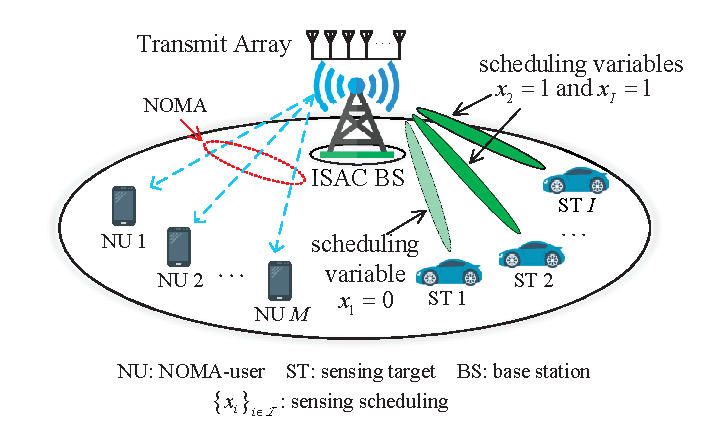
\includegraphics[width=0.96\textwidth]{figs_twc2_cld/Figure1.eps}
\caption{NOMA-assisted integrated sensing and two-tier task offloading framework}
\label{fig:figure_model51}
\end{figure*}

\subsection{System Model}

As shown in Figure \ref{fig:figure_model51}, we consider a NOMA-assisted ISTTO system including an ISCC AP with $N_t$ transmit antennas and $N_r$ receive antennas, a group of single-antenna edge computing users (ECUs) represented by $\mathcal{K}=\{1,2,...,K\}$, and a group of cloudlet servers (CSs) represented by $\mathcal{I}=\{1,2,...,I\}$. The ISCC AP performs radar sensing towards a specific target with an angle of $\theta_0$ (e.g., estimating the UAV flight data for path planning) and guarantees a sensing estimation information denoted by $Q^{\text{req}}$. Each ECU $k\in\mathcal{K}$ has a task $D_k^{\text{tot}}$ to be completed with the corresponding latency constraint $L_k^{\text{max}}$. The ISCC AP is equipped with an edge server (ES) that can provide the task offloading services for the ECUs. Moreover, the ES can further offload part of its received workloads to the CSs. Figure \ref{fig:figure_model51} demonstrates the operations of ECUs and the ISCC AP in two tiers.
\begin{itemize}
	\item In Tier-I with the duration of $t^{\text{I}}$, the ECUs offload their entire workloads to the ES. The ISCC AP transmits a sensing signal to sense the target. Meanwhile, the ISCC AP receives both the sensing echo and all ECUs' offloading signals via NOMA.
	\item In Tier-II with the duration of $t^{\text{II}}$, the ISCC AP transmits the ISAC signal via NOMA. The ISAC signal serves for two purposes, i.e., offloading part of the received workloads to multiple CSs and performing the radar sensing towards the target.
\end{itemize}

\subsection{Modeling of Tier-I}

In Tier-I, all ECUs transmit the offloading signals for offloading their respective workloads $\{D_k^{\text{tot}}\}_{k\in\mathcal{K}}$ to the ISCC AP. Meanwhile, the ISCC AP transmits a sensing signal towards a sensing target at the angle of $\theta_0$. 


\subsubsection{Signal Model}
The transmitted signal of ECU $k$ can be expressed as 
\begin{equation}
	x_k^{\text{I}}=\sqrt{p_k}s_k,
	\label{transmit_ECU_I}
\end{equation}
where $p_k$ denotes the transmit power for delivering the information symbol $s_k$ with $\mathbb{E}\{|s_k|^2\}=1$. The transmitted sensing signal of the ISCC AP in Tier-I can be expressed as
\begin{equation}
	\mathbf{x}_0^{\text{I}}=\mathbf{s}_{0}^{\text{I}},
	\label{transmit_AP_I}
\end{equation}
where $\mathbf{s}_{0}^{\text{I}}\in\mathbb{C}^{N_t\times 1}$ denotes the dedicated sensing signal with covariance $\mathbf{S}_{0}^{\text{I}}=\mathbb{E}\{\mathbf{s}_{0}^{\text{I}}(\mathbf{s}_{0}^{\text{I}})^H$\}. We next model the sensing channel for the ISCC AP regarding the sensing target. Assume that both the transmitting and receiving uniform linear arrays of the ISCC AP have half-wavelength antenna spacing. Then, the transmit steering vector and the receive steering vector on direction $\theta$ can be given by
\begin{equation}
	\mathbf{a}_t(\theta)=\frac{1}{\sqrt{N_t}}\left[1,e^{j\pi \sin\theta},...,e^{j\pi (N_t-1)\sin\theta}\right]^T,
\end{equation}
\begin{equation}
	\mathbf{a}_r(\theta)=\frac{1}{\sqrt{N_r}}\left[1,e^{j\pi \sin\theta},...,e^{j\pi (N_r-1)\sin\theta}\right]^T.
\end{equation}

We consider that there exists $M$ clutters under the angles of $\{\theta_m\}_{m=1}^{M}$, and the AP has the prior knowledge of the target and clutters. Therefore, the received signal at the AP can be expressed as 

\begin{equation}
	\begin{split}
		\mathbf{y}_{0}^{\text{I}}=&\mathop{\underbrace{\sum_{k\in\mathcal{K}}\mathbf{g}_{k}\sqrt{p_k}s_k}\limits_{\text{signal from all ECUs}}}+\mathop{\underbrace{\beta_{0}\mathbf{a}_r(\theta_{0})\mathbf{a}_t^H(\theta_{0})\mathbf{x}_{0}^{\text{I}}}\limits_{\text{sensing echo from the desired target}}}\\&+\mathop{\underbrace{\sum_{m=1}^{M}\beta_{m}\mathbf{a}_r(\theta_{m})\mathbf{a}_t^H(\theta_{m})\mathbf{x}_{0}^{\text{I}}}\limits_{\text{clutter interference}}}+\mathop{\underbrace{\mathbf{H}_{\text{SI}}\mathbf{x}_{0}^{\text{I}}+\mathbf{n}_{0}}\limits_{\text{self-interference and noise}}},
	\end{split}
	\label{receive_AP_I}
\end{equation}
where $\mathbf{g}_{k}\in\mathbb{C}^{N_r\times 1}$ denotes the channel from ECU $k$ to the ISCC AP. The complex amplitudes $\{\beta_m\}_{m=0,1,...,M}$ are primarily determined by the factors such as the path loss and radar cross-section. $\mathbf{H}_{\text{SI}}\in\mathbb{C}^{N_r\times N_t}$ denotes the residual self-interference channel at the ISCC AP. $\mathbf{n}_{0}$ denotes the noise with variance $\sigma_{0}^2$. For the sake of clear notations, we further define $\mathbf{A}_s=\beta_0\mathbf{a}_r(\theta_0)\mathbf{a}_t^H(\theta_0)$ and $\mathbf{A}_c=\sum_{m=1}^{M}\beta_m\mathbf{a}_r(\theta_m)\mathbf{a}_t^H(\theta_m)+\mathbf{H}_{\text{SI}}$.

\subsubsection{Offloading Transmission Rate and Sensing Estimation Rate}

In Tier-I, NOMA is exploited for decoding the offloading signals from the ECUs at the ISCC AP. The use of NOMA not only achieves the capacity for uplink transmission in multi-antenna systems, but also enables the ISCC AP to analyze the sensing echo in a communication-interference-free manner via the SIC, which thus reduces the inter-functionalities interference at the ISCC AP and enhances the accuracy of sensing. Without loss of any generality, we use the permutation $\Phi^{\text{I}}$ to map the decoding order of the workloads offloaded by ECU $k$ to the ISCC AP in Tier-I. For instance, $\Phi^{\text{I}}(j)<\Phi^{\text{I}}(k)$ means that the data from ECU $j$ is decoded and canceled from the received signal before decoding the data from ECU $k$. With this decoding order, based on eq. (\ref{receive_AP_I}), the achievable offloading transmission rate $R_{k}^{\text{I}}$ from ECU $k$ to the ISCC AP is given by 
\begin{equation}
	R_{k}^{\text{I}}=B^{\text{I}}\log_2\left(1+\frac{p_k\mathbf{c}_{k}^H\mathbf{g}_{k}\mathbf{g}_{k}^H\mathbf{c}_{k}}{\mathbf{c}_{k}^H\mathbf{\Gamma}_{k}\mathbf{c}_{k}}\right), \forall k\in\mathcal{K},
	\label{R_k_I}
\end{equation}
where $B^{\text{I}}$ denotes the transmission channel bandwidth in Tier-I, and $\mathbf{c}_{k}\in\mathbb{C}^{N_r\times 1}$ denotes the ISCC AP's communication receive beamforming. In eq. (\ref{R_k_I}), $\mathbf{\Gamma}_{k}$ denotes the total interference for receiving ECU $k$'s data, and it can be expressed as
\vspace{0.5cm}

\begin{equation}
	\mathbf{\Gamma}_{k}=\sum_{\Phi^{\text{I}}(j)>\Phi^{\text{I}}(k)}\hspace{-0.3cm}p_j\mathbf{g}_{j}\mathbf{g}_{j}^H+\mathbf{A}_s\mathbf{S}_{0}^{\text{I}}\mathbf{A}_s^H+\mathbf{A}_c\mathbf{S}_{0}^{\text{I}}\mathbf{A}_c^H+\sigma_{0}^2\mathbf{I}_N.
\end{equation}
According to \cite{twc1.van2002optimum}, the optimal receiver $\mathbf{c}_{k}^\ast$ is given by 
\begin{equation}
	\mathbf{c}_{k}^\ast=\arg\max\frac{p_k\mathbf{c}_{k}^H\mathbf{g}_{k}\mathbf{g}_{k}^H\mathbf{c}_{k}}{\mathbf{c}_{k}^H\mathbf{\Gamma}_{k}\mathbf{c}_{k}}=\mathbf{\Gamma}_{k}^{-1}\mathbf{g}_{k}, \forall k\in\mathcal{K}.
\end{equation}
By substituting $\mathbf{c}_{k}^\ast$ into eq. (\ref{R_k_I}), the achievable offloading transmission rate $R_{k}^{\text{I}}$ can be rewritten as
\begin{equation}
	R_{k}^{\text{I}}=B^{\text{I}}\log_2\left(1+p_k\mathbf{g}_{k}^H\mathbf{\Gamma}_{k}^{-1}\mathbf{g}_{k}\right), \forall k\in\mathcal{K}.
	\label{R_k_I_re}
\end{equation}
With the duration of $t^{\text{I}}$ in Tier-I, the offloading transmission rate $R_{k}^{\text{I}}$ should satisfy
\vspace{-0.4cm}
\begin{equation}
	t^{\text{I}}R_{k}^{\text{I}}=D_k^{\text{tot}}, \forall k\in\mathcal{K}.
	\label{satisfy_I}
\end{equation}

\vspace{-0.6cm}
We utilize the sensing estimation rate to measure the radar sensing performance, which is defined as the cancellation of the uncertainty in the target parameters per second. Based on eq. (\ref{receive_AP_I}), after decoding the transmission signal from all ECUs, the sensing estimation rate $Q^{\text{I}}$ of the ISCC AP for sensing the target in Tier-I is
\begin{equation}
	Q^{\text{I}}=\frac{\delta}{2\mu}\log_2\left(1+\frac{2\mu B^{\text{I}}\mathbf{u}^H\mathbf{A}_s\mathbf{S}_{0}^{\text{I}}\mathbf{A}_s^H\mathbf{u}}{\mathbf{u}^H\mathbf{\Lambda}\mathbf{u}}\right),
	\label{sensing_I}
\end{equation}
where $\delta$ represents the duty factor, and $\mu$ represents the pulse duration. Vector $\mathbf{u}$ denotes the ISCC AP's sensing receive beamforming. In eq. (\ref{sensing_I}), $\mathbf{\Lambda}$ denotes the total interference of the ISCC AP for sensing the target in Tier-I, and it can be expressed as
\vspace{-0.1cm}
\begin{equation}
		\mathbf{\Lambda}=\mathbf{A}_c\mathbf{S}_{0}^{\text{I}}\mathbf{A}_c^H+\sigma_{0}^2\mathbf{I}_N.
\end{equation}

According to \cite{twc1.van2002optimum}, the optimal receiver $\mathbf{u}^\ast$ is given by 
\begin{equation}
	\mathbf{u}^\ast=\arg\max\frac{\mathbf{u}^H\mathbf{A}_s\mathbf{S}_{0}^{\text{I}}\mathbf{A}_s^H\mathbf{u}}{\mathbf{u}^H\mathbf{\Lambda}\mathbf{u}}=\mathbf{\Lambda}^{-1}\mathbf{a}_r(\theta_0). \label{optimal_receive}
\end{equation}
By substituting $\mathbf{u}^\ast$ into eq. (\ref{sensing_I}), we can rewrite $Q^{\text{I}}$ as
\vspace{-0.3cm}
\begin{equation}
	Q^{\text{I}}=\frac{\delta}{2\mu}\log_2(1+2\mu B^{\text{I}}(\mathbf{s}_0^{\text{I}})^H\mathbf{A}_s^H\mathbf{\Lambda}^{-1}\mathbf{A}_s\mathbf{s}_0^{\text{I}}).
	\label{sensing_I_re}
\end{equation}

\subsection{Modeling of Tier-II}

After the ISCC AP receives the workloads from all ECUs, in Tier-II, the ISCC AP offloads part of its received workloads to multiple CSs and performs the radar sensing simultaneously.

\subsubsection{Signal model}
The transmitted ISAC signal of the ISCC AP in Tier-II can be expressed as
\begin{equation}
	\mathbf{x}_0^{\text{II}}=\sum_{i\in\mathcal{I}}\mathbf{w}_iz_i+\mathbf{s}_{0}^{\text{II}},
	\label{transmit_AP_II}
\end{equation}
where $\mathbf{w}_i\in\mathbb{C}^{N_t\times 1}$ denotes the transmit beamforming for CS $i$ and $z_i$ with $\mathbb{E}\{|z_i|^2\}=1$ denotes the symbol for CS $i$. Meanwhile, in eq. (\ref{transmit_AP_II}), $\mathbf{s}_0^{\text{II}}$ denotes a dedicated sensing signal with covariance $\mathbf{S}_0^{\text{II}}=\mathbb{E}\{\mathbf{s}_0^{\text{II}}(\mathbf{s}_0^{\text{II}})^H\}$ for achieving the enhanced sensing performance in the scenario of multiple downlink users.
The received signal at CS $i$ is given by
\begin{equation}
	y_i^{\text{II}}=\mathbf{h}_i^H\mathbf{w}_iz_i+\sum_{j\in\mathcal{I},j\neq i}\mathbf{h}_i^H\mathbf{w}_jz_j+\mathbf{h}_i^H\mathbf{s}_{0}^{\text{II}}+n_i,
	\label{receive_CS_II}
\end{equation}
where $\mathbf{h}_i\in\mathbb{C}^{N_t\times 1}$ denotes the channel gain between the ISCC AP and CS $i$, and $n_i$ denotes the noise with variance $\sigma_i^2$. The received signal at the ISCC AP in Tier-II is given by
\begin{equation}
	\mathbf{y}_0^{\text{II}}=\mathbf{A}_s\mathbf{x}_0^{\text{II}}+\mathbf{A}_c\mathbf{x}_0^{\text{II}}+\mathbf{n}_0.
	\label{receive_AP_II}
\end{equation}

\subsubsection{Offloading Transmission Rate and Sensing Estimation Rate}
In Tier-II, the ISCC AP exploits the downlink NOMA ISAC signal for sensing the target and offloading part of its received workloads to different cloudlet servers simultaneously. However, the dedicated sensing signal impairs the communication performance from the ISCC AP to CSs. To address this issue, we design a NOMA decoding scheme which can remove the interference from the dedicated sensing signal to the downlink offloading signals. In particular, to guarantee that the dedicated sensing signal is decoded before decoding the communication signals, the following condition should be satisfied

\begin{equation}
	|\mathbf{h}_i^H\mathbf{s}_0^{\text{II}}|^2\ge|\mathbf{h}_i^H\mathbf{w}_i|^2, \forall i\in\mathcal{I}.
	\label{condition}
\end{equation}
We use the permutation $\Phi^{\text{II}}$ to map the decoding order of the workloads offloaded by the ISCC AP to the CSs. After removing the interference from the dedicated sensing signal, based on eq. (\ref{receive_CS_II}), the offloading transmission rate $R_i^{\text{II}}$ achieved by CS $i$ can be expressed as 
\begin{equation}
	R_i^{\text{II}}=B^{\text{II}}\log_2\left(1+\frac{|\mathbf{h}_i^H\mathbf{w}_i|^2}{\sum_{\Phi^{\text{II}}(j)>\Phi^{\text{II}}(i)}|\mathbf{h}_i^H\mathbf{w}_j|^2+\sigma_i^2}\right), \forall i\in\mathcal{I},
	\label{R_i_II}
\end{equation}
where $B^{\text{II}}$ denotes the transmission channel bandwidth in Tier-II. We use $d_{ki}$ to denote the ECU $k$'s workloads offloaded from the ISCC AP to CS $i$, with the duration of $t^{\text{II}}$ in Tier-II, $R_i^{\text{II}}$ should satisfy
\begin{equation}
	t^{\text{II}}R_{i}^{\text{II}} \ge \sum_{k\in\mathcal{K}}d_{ki}, \forall i\in\mathcal{I}.
	\label{satisfy_II}
\end{equation}
Similar to eq. (\ref{sensing_I_re}), the sensing estimation rate $Q^{\text{II}}$ of the ISCC AP for sensing the target in Tier-II can be expressed as
\begin{equation}
	Q^{\text{II}}=\frac{\delta}{2\mu}\log_2\Big(1+2\mu B^{\text{II}}(\mathbf{x}_0^{\text{II}})^H\mathbf{A}_s^H\mathbf{\Psi}^{-1}\mathbf{A}_s\mathbf{x}_0^{\text{II}}\Big),
	\label{sensing_II}
\end{equation}
where $\mathbf{\Psi}$ denotes the total interference of the ISCC AP for sensing the target in Tier-II, and it can be expressed as
\begin{equation}
	\mathbf{\Psi}=\mathbf{A}_c\mathbf{x}_0^{\text{II}}(\mathbf{x}_0^{\text{II}})^H\mathbf{A}_c^H+\sigma_0^2\mathbf{I}_N.
\end{equation}



\subsection{Modeling of Latency and Energy Consumption}
The energy consumption of ECU $k$ for its offloading transmission is given by
\begin{equation}
	E_k^{\text{off}}=p_kt^{\text{I}}, \forall k\in\mathcal{K}.
	\label{energy_ECU_offloading}
\end{equation}
For ECU $k$, the latency for completing its workloads is determined by two parts, including the latency $l_k^{\text{ES}}$ for processing at the ES, and the latency $l_k^{\text{CS}}$ for processing at the CSs. 
The latency for processing ECU $k$'s workloads at the ES can be expressed as
\begin{equation}
	l_k^{\text{ES}}=t^{\text{I}}+\frac{\upsilon_k(D_k^{\text{tot}}-\sum_{i\in\mathcal{I}}d_{ki})}{\varrho_k}, \forall k\in\mathcal{K},
	\label{latency_ES}
\end{equation}
where $\upsilon_k$ denotes the number of CPU cycles for processing one bit of $D_k^{\text{tot}}$ and $\varrho_k$ denotes the ES's processing-rate allocated for processing ECU $k$'s offloaded workloads. The ES's energy consumption for processing ECU $k$'s workloads can be expressed as
\begin{equation}
	E_k^{\text{ES}}=\epsilon\varrho_k^2\upsilon_k(D_k^{\text{tot}}-\sum_{i\in\mathcal{I}}d_{ki}), \forall k\in\mathcal{K},
	\label{energy_ES_computing}
\end{equation}
where $\epsilon$ is the power consumption coefficient of the ES. The energy consumption of the ISCC AP for performing sensing in Tier-I and further offloading to the CSs while performing sensing in Tier-II is given by
\begin{equation}
	E^{\text{AP}}=\textbf{Tr}\left(\mathbf{S}_0^{\text{I}}\right)t^{\text{I}}+\textbf{Tr}\left(\sum_{i\in\mathcal{I}}\mathbf{w}_i\mathbf{w}_i^H+\mathbf{S}_0^{\text{II}}\right)t^{\text{II}}.
	\label{energy_AP_sensing_offloading}
\end{equation}

The latency for processing ECU $k$'s workloads at the CSs can be expressed as
\begin{equation}
	l_k^{\text{CS}}=t^{\text{I}}+t^{\text{II}}+\max_i\{\frac{\upsilon_kd_{ki}}{\varsigma_{ki}}\}, \forall k\in\mathcal{K},
	\label{latency_CS}
\end{equation}
where $\varsigma_{ki}$ denotes the CS $i$'s processing-rate allocated for processing the offloaded workloads from ECU $k$.

Based on the above modelings, the total latency $l_k$ for completing ECU $k$'s workloads is given by
\begin{equation}
	l_k=\max\{l_k^{\text{ES}}, l_k^{\text{CS}}\}, \forall k\in\mathcal{K}.
	\label{latency_k}
\end{equation}
The total energy consumption of the ECUs and the ISCC AP with the ES is given by
\begin{equation}
	E^{\text{tot}}=\mathop{\underbrace{\sum_{k\in\mathcal{K}}E_k^{\text{off}}}\limits_{\text{ECUs}}}+\mathop{\underbrace{E^{\text{AP}}+\sum_{k\in\mathcal{K}}E_k^{\text{ES}}}\limits_{\text{ISCC AP and ES}}}.
	\label{energy_total}
\end{equation}
\vspace{1cm}

\subsection{Problem Formulation}
We focus on an energy-minimization design (EMD) for the ECUs and the ISCC AP with the ES, including all ECUs' offloading energy consumption in Tier-I, the ES's local processing energy consumption, and the energy consumption of the ISCC AP for performing the radar sensing in Tier-I and further offloading to the CSs while performing sensing in Tier-II. 
To accomplish this objective, we jointly optimize the transmit beamforming $\{\mathbf{w}_{i}\}_{i\in\mathcal{I}}$, the dedicated sensing signals $\mathbf{s}_{0}^{\text{I}}$ and $\mathbf{s}_{0}^{\text{II}}$, the ECUs' transmit powers $\{p_k\}_{k\in\mathcal{K}}$, the two-tier durations $t^{\text{I}}$ and $t^{\text{II}}$, the Tier-II offloading data volume $\{d_{ki}\}_{k\in\mathcal{K},i\in\mathcal{I}}$, and the ES's processing-rate $\{\varrho_k\}_{k\in\mathcal{K}}$ as follows.
\begin{flalign}
	\text{(EMD):~}
	&\min  E^{\text{tot}}\nonumber\\
	\text{subject to:~}
	& \text{constraints~}(\ref{satisfy_I}), (\ref{condition}), \text{~and~}(\ref{satisfy_II}), \nonumber
	\\
	&l_k \le L_k^{\text{max}}, \forall k\in\mathcal{K}, \label{con1}
	\\
	&p_k \le P_k^{\text{max}}, \forall k\in\mathcal{K}, \label{con2}
	\\
	&\textbf{Tr}\left(\mathbf{S}_0^{\text{I}}\right) \le P^{\text{AP,max}}, \label{con3}
	\\
	&\textbf{Tr}\left(\sum_{i\in\mathcal{I}}\mathbf{w}_i\mathbf{w}_i^H+\mathbf{S}_0^{\text{II}}\right) \le P^{\text{AP,max}}, \label{con4}
	\\
	&0 \le \sum_{i\in\mathcal{I}}d_{ki} \le D_k^{\text{max}}, \forall k\in\mathcal{K}, \label{con5}
	\\
	&0 \le t^{\text{I}} \le T^{\text{max}}, \label{con6}
	\\
	&0 \le t^{\text{II}} \le T^{\text{max}}, \label{con7}
	\\
	&t^{\text{I}}Q^{\text{I}}+t^{\text{II}}Q^{\text{II}} \ge Q^{\text{req}}, \label{con8}
	\\
	&0 \le \sum_{k\in\mathcal{K}}\varrho_k \le \varrho^{\text{max}}, \label{con9}
	\\
	\text{variables:~} & \{\mathbf{w}_{i}\}_{i\in\mathcal{I}}, \mathbf{s}_{0}^{\text{I}}, \mathbf{s}_{0}^{\text{II}}, \{p_k\}_{k\in\mathcal{K}}, t^{\text{I}}, t^{\text{II}},  \{d_{ki}\}_{k\in\mathcal{K},i\in\mathcal{I}}, \text{~and~} \{\varrho_k\}_{k\in\mathcal{K}}.\nonumber
\end{flalign}
Constraint (\ref{con1}) guarantees that the overall latency in completing ECU $k$'s workloads cannot exceed the latency requirement $L_k^{\text{max}}$. Constraint (\ref{con2}) provides an upper bound for ECU $k$'s transmit power. Constraints (\ref{con3}) and (\ref{con4}) ensure that ISCC AP's transmit power cannot exceed its power capacity $P^{\text{AP,max}}$. Constraint (\ref{con5}) guarantees that the tasks of ECU $k$ offloaded from the ES to the CSs cannot exceed those offloaded to the ES. Constraints (\ref{con6}) and (\ref{con7}) mean that both Tier-I duration and Tier-II duration cannot exceed a specified upper-bound $T^{\text{max}}$ (i.e., the duration for occupying the radio interface). Constraint (\ref{con8}) guarantees the required sensing estimation information $Q^{\text{req}}$ over the total duration $t^{\text{I}}+t^{\text{II}}$. Constraint (\ref{con9}) implies that the ES's total allocated processing-rate for all ECUs cannot exceed its computing capacity $\varrho^{\text{max}}$.



\section{Proposed Algorithms for Problem (EMD)} \label{chap5_sec_solution_Joint}

\subsection{Problem Reformulation}

It can be found that Problem (EMD) is a strictly non-convex optimization problem. Thus, it is very difficult to solve Problem (EMD) directly. To this end, we first reformulate Problem (EMD) to obtain its equivalent form.

By putting eq. (\ref{R_k_I_re}) into constraint (\ref{satisfy_I}), we derive
\begin{equation}
	p_k(t^{\text{I}},\mathbf{S}_0^{\text{I}})=\left(\mathbf{g}_k^H\mathbf{\Omega}^{-1}\mathbf{g}_k\right)^{-1}\left(2^{\frac{D_k^{\text{tot}}}{t^{\text{I}}B^{\text{I}}}}-1\right)2^{\frac{\sum_{\Phi^{\text{I}}(j)>\Phi^{\text{I}}(k)}D_j^{\text{tot}}}{t^{\text{I}}B^{\text{I}}}}, 
	\label{p_k}
\end{equation}
where 
\begin{equation}
	\mathbf{\Omega}=\mathbf{A}_s\mathbf{S}_{0}^{\text{I}}\mathbf{A}_s^H+\mathbf{A}_c\mathbf{S}_{0}^{\text{I}}\mathbf{A}_c^H+\sigma_{0}^2\mathbf{I}_N.
	\label{pure noise}
\end{equation}

\begin{proposition}
	\label{proposition11}
	The optimal solution of $\{\varrho_k\}_{k\in\mathcal{K}}$ is given by
	\begin{equation}
		\varrho_k^\ast=\frac{\upsilon_k(D_k^{\mathrm{tot}}-\sum_{i\in\mathcal{I}}d_{ki})}{L_k^{\mathrm{max}}-t^{\mathrm{I}}}, \forall k\in\mathcal{K}.
		\label{varrho_optimal}
	\end{equation}
\end{proposition}
\begin{proof}
	With eq. (\ref{latency_k}), constraint (\ref{con1}) can be transformed into 
\begin{equation}
	\frac{\upsilon_k(D_k^{\text{tot}}-\sum_{i\in\mathcal{I}}d_{ki})}{L_k^{\text{max}}-t^{\text{I}}} \le \varrho_k, \forall k\in\mathcal{K},
	\label{latency_transformed_1}
\end{equation}
\begin{equation}
	\frac{\upsilon_kd_{ki}}{\varsigma_{ki}} \le L_k^{\text{max}}-t^{\text{I}}-t^{\text{II}}, \forall k\in\mathcal{K}, i\in\mathcal{I}.
	\label{latency_transformed_2}
\end{equation}	
It can be identified that the objective function of Problem (EMD) increases monotonically with respect to $\{\varrho_k\}_{k\in\mathcal{K}}$. Therefore, in the feasible solution interval, minimizing the total energy consumption is equivalent to finding the minimum value of $\{\varrho_k\}_{k\in\mathcal{K}}$. According to the lower-bounds given in eq. (\ref{latency_transformed_1}), the optimal values of $\{\varrho_k\}_{k\in\mathcal{K}}$ are given in eq. (\ref{varrho_optimal}).
\end{proof}

With the optimal solution of $\{\varrho_k\}_{k\in\mathcal{K}}$, we can rewrite eq. (\ref{energy_ES_computing}) as
\begin{equation}
	E_k^{\text{ES}}=\frac{\epsilon\upsilon_k^3(D_k^{\text{tot}}-\sum_{i\in\mathcal{I}}d_{ki})^3}{({L_k^{\text{max}}-t^{\text{I}}})^2}, \forall k\in\mathcal{K}.
	\label{energy_ES_computing_re}
\end{equation}
After the above operations, Problem (EMD) can be equivalently transformed into Problem (EMD-E) as follows.
\begin{flalign}
	\text{(EMD-E):~}
	&\min  E^{\text{tot}}\nonumber\\
	\text{subject to:~}
	& \text{constraints~} (\ref{condition}), (\ref{satisfy_II}), (\ref{con3}), (\ref{con4}), (\ref{con5}), (\ref{con6}),\nonumber \\& (\ref{con7}), \text{~and~} (\ref{con8}), \nonumber
	\\
	&p_k(t^{\text{I}},\mathbf{S}_0^{\text{I}}) \le P_k^{\text{max}}, \forall k\in\mathcal{K}, \label{equ_con1}
	\\
	&0 \le \sum_{k\in\mathcal{K}}\frac{\upsilon_k(D_k^{\text{tot}}-\sum_{i\in\mathcal{I}}d_{ki})}{L_k^{\text{max}}-t^{\text{I}}} \le \varrho^{\text{max}}, \label{equ_con2}
	\\
	&\frac{\upsilon_kd_{ki}}{\varsigma_{ki}} \le L_k^{\text{max}}-t^{\text{I}}-t^{\text{II}}, \forall k\in\mathcal{K}, i\in\mathcal{I}, \label{equ_con3}
	\\
	\text{variables:~} & \{\mathbf{w}_{i}\}_{i\in\mathcal{I}}, \mathbf{s}_{0}^{\text{I}}, \mathbf{s}_{0}^{\text{II}}, t^{\text{I}}, t^{\text{II}}, \text{~and~} \{d_{ki}\}_{k\in\mathcal{K},i\in\mathcal{I}}.\nonumber
\end{flalign}


\subsection{Decomposition of Problem (EMD-E)}

Problem (EMD-E) is still a strictly non-convex optimization problem. To address this difficulty, we propose the following decomposition approach.


1) Bottom-problem under the given $t^{\text{II}}$: Given the duration $t^{\text{II}}$ of Tier-II, Problem (EMD-E) turns into Problem (EMD-BOT) as follows.
\begin{flalign}
	\text{(EMD-BOT):~}
	&E^{\text{tot,min}} = \min  E^{\text{tot}}\nonumber\\
	\text{subject to:~}
	& \text{constraints~} (\ref{condition}), (\ref{satisfy_II}), (\ref{con3}), (\ref{con4}), (\ref{con5}), (\ref{con6}),\nonumber \\& (\ref{con8}), (\ref{equ_con1}), (\ref{equ_con2}), \text{~and~} (\ref{equ_con3}), \nonumber
	\\
	\text{variables:~} & \{\mathbf{w}_{i}\}_{i\in\mathcal{I}}, \mathbf{s}_{0}^{\text{I}}, \mathbf{s}_{0}^{\text{II}}, t^{\text{I}}, \text{~and~} \{d_{ki}\}_{k\in\mathcal{K},i\in\mathcal{I}}.\nonumber
\end{flalign}

2) Top-problem to optimize $t^{\text{II}}$: After solving Problem (EMD-BOT) and obtaining the value of $E^{\text{tot,min}}$ with the given $t^{\text{II}}$, we then continue to optimize $t^{\text{II}}$, which results in the following optimization problem.
\begin{flalign}
	\text{(EMD-TOP):~}
	&\min  E^{\text{tot,min}}\nonumber\\
	\text{subject to:~}
	& \text{constraint~} (\ref{con7}), \nonumber
	\\
	\text{variable:~} & t^{\text{II}}.\nonumber
\end{flalign}


\subsection{Decomposition of Problem (EMD-BOT)}

In Problem (EMD-BOT), the duration $t^{\text{I}}$ of Tier-I, the dedicated sensing signals $\mathbf{s}_{0}^{\text{I}}$ and $\mathbf{s}_{0}^{\text{II}}$, and the transmit beamforming $\{\mathbf{w}_{i}\}_{i\in\mathcal{I}}$ show a strong coupling effect in both the objective function and constraints. To solve Problem (EMD-BOT) efficiently, we propose the following decomposition of Problem (EMD-BOT) based on the block coordinated descent (BCD) method.

1) Sub-problem to optimize $t^{\text{I}}$ under the given $\{\mathbf{w}_{i}\}_{i\in\mathcal{I}}$, $\mathbf{s}_{0}^{\text{I}}$, $\mathbf{s}_{0}^{\text{II}}$, and $\{d_{ki}\}_{k\in\mathcal{K},i\in\mathcal{I}}$.
\begin{flalign}
	\text{(Sub-t):~}
	&\min  E^{\text{tot}}\nonumber\\
	\text{subject to:~}
	& \text{constraints~} (\ref{con6}), (\ref{con8}), (\ref{equ_con1}), (\ref{equ_con2}), \text{~and~} (\ref{equ_con3}), \nonumber
	\\
	\text{variable:~} & t^{\text{I}}.\nonumber
\end{flalign}

2) Sub-problem to optimize $\{\mathbf{w}_{i}\}_{i\in\mathcal{I}}$, $\mathbf{s}_{0}^{\text{II}}$, and $\{d_{ki}\}_{k\in\mathcal{K},i\in\mathcal{I}}$ under the given $t^{\text{I}}$ and $\mathbf{s}_{0}^{\text{I}}$.
\begin{flalign}
	\text{(Sub-w):~}
	&\min  E^{\text{tot}}\nonumber\\
	\text{subject to:~}
	& \text{constraints~} (\ref{condition}), (\ref{satisfy_II}), (\ref{con4}), (\ref{con5}), (\ref{con8}),  (\ref{equ_con2}), \text{~and~} (\ref{equ_con3}), \nonumber
	\\
	\text{variables:~} & \{\mathbf{w}_{i}\}_{i\in\mathcal{I}}, \mathbf{s}_{0}^{\text{II}}, \text{~and~} \{d_{ki}\}_{k\in\mathcal{K},i\in\mathcal{I}}.\nonumber
\end{flalign}

3) Sub-problem to optimize $\mathbf{s}_{0}^{\text{I}}$ under the given $t^{\text{I}}$, $\{\mathbf{w}_{i}\}_{i\in\mathcal{I}}$, $\mathbf{s}_{0}^{\text{II}}$, and $\{d_{ki}\}_{k\in\mathcal{K},i\in\mathcal{I}}$.
\begin{flalign}
	\text{(Sub-s):~}
	&\min  E^{\text{tot}}\nonumber\\
	\text{subject to:~}
	& \text{constraints~} (\ref{con3}), (\ref{con8}), \text{~and~} (\ref{equ_con1}), \nonumber
	\\
	\text{variable:~} & \mathbf{s}_{0}^{\text{I}}.\nonumber
\end{flalign}
According to the criterion of the BCD method, the three sub-problems (i.e., Problem (Sub-t), Problem (Sub-w) and Problem (Sub-s)) are solved iteratively to obtain the solution of Problem (EMD-BOT). The key advantage of using the above decomposition lies in that we can solve the subproblem optimally in an individual manner.
		

\subsection{Proposed Algorithm for Solving Problem (Sub-t)}

Although Problem (Sub-t) is still non-convex, we have an observation regarding its objective function as follows.
\begin{proposition}
	\label{proposition12}
	The objective function of Problem (Sub-t) is the difference between two monotonic functions with respect to $t^{\mathrm{I}}$.
\end{proposition}
\begin{proof}
	The objective function of Problem (Sub-t) consists of three parts, i.e., all ECUs' energy consumption $\sum_{k\in\mathcal{K}}E_k^{\text{off}}$ for offloading, the ISCC AP's energy consumption $E^{\text{AP}}$ within two tiers, and ES's energy consumption $\sum_{k\in\mathcal{K}}E_k^{\text{ES}}$ for processing. According to eq. (\ref{energy_AP_sensing_offloading}) and eq. (\ref{energy_ES_computing_re}), it can be observed that $E^{\text{AP}}$ and $\sum_{k\in\mathcal{K}}E_k^{\text{ES}}$ are increasing with respect to $t^{\text{I}}$. Next we show that $\sum_{k\in\mathcal{K}}E_k^{\text{off}}$ is decreasing with respect to $t^{\text{I}}$.

The first derivative of $E_k^{\text{off}}$ with respect to $t^{\text{I}}$ can be expressed as
\begin{equation}
	\begin{split}
	\frac{\mathrm{d}E_k^{\text{off}}}{\mathrm{d}t^{\text{I}}}&=2^{\frac{\sum_{\Phi^{\text{I}}(j)\ge\Phi^{\text{I}}(k)}D_j^{\text{tot}}}{t^{\text{I}}B^{\text{I}}}}\left(1-\frac{\sum_{\Phi^{\text{I}}(j)\ge\Phi^{\text{I}}(k)}D_j^{\text{tot}}}{t^{\text{I}}B^{\text{I}}}\ln2\right)\\&-2^{\frac{\sum_{\Phi^{\text{I}}(j)>\Phi^{\text{I}}(k)}D_j^{\text{tot}}}{t^{\text{I}}B^{\text{I}}}}\left(1-\frac{\sum_{\Phi^{\text{I}}(j)>\Phi^{\text{I}}(k)}D_j^{\text{tot}}}{t^{\text{I}}B^{\text{I}}}\ln2\right).
	\end{split}
	\label{derivative_E}
\end{equation}	
Let $f^{'}=2^q(1-q\ln2)$. By the first derivative of $f^{'}$ with respect to $q$, we can discover that
\begin{equation}
	\frac{\mathrm{d}f^{'}}{\mathrm{d}q}=-q2^q(\ln2)^2<0,
	\label{derivative_f}
\end{equation}
which means $f^{'}$ is decreasing with respect to $q$. With eq. (\ref{derivative_f}), we can derive that 
\begin{equation}
	\frac{\mathrm{d}E_k^{\text{off}}}{\mathrm{d}t^{\text{I}}}<0,
	\label{derivative_E_derive}
\end{equation}
which proves that $\sum_{k\in\mathcal{K}}E_k^{\text{off}}$ is decreasing with respect to $t^{\text{I}}$. Thus, we can rewrite the objective function of Problem (Sub-t) as 

\begin{equation}
	E^{\text{tot}}=E^{\text{AP}}+\sum_{k\in\mathcal{K}}E_k^{\text{ES}}-(-\sum_{k\in\mathcal{K}}E_k^{\text{off}}),
	\label{difference}
\end{equation}
which is the difference between two monotonically increasing functions with respect to $t^{\text{I}}$.
\end{proof}

With the hidden monotonic feature of Problem (Sub-t) in Proposition \ref{proposition12}, we can establish Problem (Sub-t) as a canonical monotonic optimization form by introducing an auxiliary variable $\alpha^{\text{dif}}$ and a new function $F(t^{\text{I}},\alpha^{\text{dif}})$. For the sake of clear expression, we define
\begin{equation}
	f(t^{\text{I}})=E^{\text{AP}}+\sum_{k\in\mathcal{K}}E_k^{\text{ES}}.
	\label{f}
\end{equation}
According to Proposition \ref{proposition12} and constraint (\ref{con6}), we have 
\begin{equation}
	f(t^{\text{I}}) \le E^{\text{max}} = f(T^{\text{max}}).
	\label{le}
\end{equation}
Then, $\alpha^{\text{dif}}$ and $F(t^{\text{I}},\alpha^{\text{dif}})$ can be respectively defined as 
\begin{equation}
	\alpha^{\text{dif}}=E^{\text{max}}-f(t^{\text{I}}),
	\label{diff}
\end{equation}
\begin{equation}
	F(t^{\text{I}},\alpha^{\text{dif}})=-\sum_{k\in\mathcal{K}}E_k^{\text{off}}+\alpha^{\text{dif}}.
	\label{F}
\end{equation}

After the above operations, we can derive the following equivalent form of Problem (Sub-t).
\begin{flalign}
	\text{(MO-t):~}
	&\max  F(t^{\text{I}},\alpha^{\text{dif}})\nonumber\\
	\text{subject to:~}
	& \text{constraints~} (\ref{con6}), (\ref{con8}), (\ref{equ_con1}), (\ref{equ_con2}), \text{and~} (\ref{equ_con3}), \nonumber
	\\
	&0\le \alpha^{\text{dif}} \le E^{\text{max}}-f(t^{\text{I}}), \label{trans_diff}
	\\
	\text{variables:~} & t^{\text{I}} \text{~and~} \alpha^{\text{dif}}.\nonumber
\end{flalign}


In Problem (MO-t), we transform eq. (\ref{diff}) of $\alpha^{\text{dif}}$ into constraint (\ref{trans_diff}) to establish a canonical monotonic optimization problem. Nevertheless, in our Algorithm-PA below, the intersection can be obtained on the upper boundary with bisection search in Step 5, which means that $\alpha^{\text{dif}}$ always achieves its maximum value, i.e., $\alpha^{\text{dif}}=E^{\text{max}}-f(t^{\text{I}})$. Therefore, the transformation from eq. (\ref{diff}) to constraint (\ref{trans_diff}) does not change the optimality of the problem.


\begin{proposition}
	\label{proposition13}
	Problem (MO-t) is a canonical form of monotonic optimization problem with respect to $t^{\mathrm{I}}$ and $\alpha^{\mathrm{dif}}$.
\end{proposition}
\begin{proof}
	The proof is based on the monotonic optimization theory. Specifically, the objective function is increasing in $(t^{\text{I}},\alpha^{\text{dif}})$. Moreover, the feasible region is the intersection of a normal set (defined in eq. (\ref{normal})) and a conormal set (defined in eq. (\ref{conormal})). Therefore, Problem (MO-t) is a canonical monotonic optimization form \cite{twc2.zhang2013monotonic,twc2.tuy2000monotonic}.
\end{proof}

\begin{algorithm}
	\caption{: To solve Problem (Sub-t) and obtain optimal $t^{\text{I},\ast}$.}
	\begin{algorithmic}[1]
		\STATE  \textbf{Initialization:} Initialize the vertex set $\mathcal{V}^0=\{(T^{\text{max}},E^{\text{max}})\}$. Set the current best value $\text{CBV}^0=-\infty$ and the current best solution $\mathbf{CBS}^0$ as an empty set. Set the iteration number $\tau=0$. Set $\xi_1$ as a very small positive number.
		\REPEAT
		\STATE Update $\tau=\tau+1$.
		\STATE Find the vertex $\mathbf{z}^\tau=\arg\max\{F(t^{\text{I}},\alpha^{\text{dif}})|(t^{\text{I}},\alpha^{\text{dif}})\in\mathcal{V}^{\tau-1}\}$ from $\mathcal{V}^{\tau-1}$.
		\STATE Use bisection search to find the projection of $\mathbf{z}^\tau$ on the boundary of $\mathcal{M}$, which is denoted as $\pi_{\mathcal{M}}(\mathbf{z}^\tau)$.
		\IF{$|\pi_{\mathcal{M}}(\mathbf{z}^\tau)-\mathbf{z}^\tau|\le\xi_1$}
		\STATE Update $\mathbf{CBS}^\tau=\mathbf{z}^\tau$ and $\text{CBV}^\tau=F(\mathbf{z}^\tau)$.
		\ELSE
		\IF{$\pi_{\mathcal{M}}(\mathbf{z}^\tau)\in\mathcal{M}\cap\mathcal{N}$ and $F(\pi_{\mathcal{M}}(\mathbf{z}^\tau))\ge\text{CBV}^{\tau-1}$}
		\STATE Update $\mathbf{CBS}^\tau=\pi_{\mathcal{M}}(\mathbf{z}^\tau)$ and $\text{CBV}^\tau=F(\pi_{\mathcal{M}}(\mathbf{z}^\tau))$.
		\ELSE
		\STATE Update $\mathbf{CBS}^\tau=\mathbf{CBS}^{\tau-1}$ and $\text{CBV}^\tau=\text{CBV}^{\tau-1}$.
		\ENDIF
		\STATE Set $\mathbf{z}^{\text{temp}}=\pi_{\mathcal{M}}(\mathbf{z}^\tau)$ and update $\mathcal{V}^\tau=\{\mathcal{V}^{\tau-1}\backslash\mathbf{z}^\tau\}\cup\{(\mathbf{z}^\tau(1),\mathbf{z}^{\text{temp}}(2)),(\mathbf{z}^{\text{temp}}(1),\mathbf{z}^\tau(2))\}$.
		\STATE Remove from $\mathcal{V}^\tau$ the improper vertices and the vertices $\{\mathbf{v}\in\mathcal{V}^\tau|\mathbf{v}\notin\mathcal{N}\}$.
		\ENDIF
		\UNTIL $|F(\mathbf{z}^\tau)-\mathbf{CBV}^\tau| \le \xi_1$.
		\STATE \textbf{Output:} Output the optimal solution $(t^{\text{I},\ast},\alpha^{\text{dif},\ast})=\mathbf{CBS}_j$ for Problem (MO-t). Notice that $t^{\text{I},\ast}$ is also the solution for Problem (Sub-t).
	\end{algorithmic}
\end{algorithm}	

Based on the monotonicity in constraints (\ref{con6}), (\ref{con8}), (\ref{equ_con1}), (\ref{equ_con2}), (\ref{equ_con3}) and (\ref{trans_diff}), we can establish the following normal set $\mathcal{M}$ and conormal set $\mathcal{N}$.
\begin{equation}
	\mathcal{M}=\{(t^{\text{I}},\alpha^{\text{dif}})|\text{Constraints~} (\ref{con6}), (\ref{equ_con2}), (\ref{equ_con3}), (\ref{trans_diff})\},
	\label{normal}
\end{equation}
\begin{equation}
	\mathcal{N}=\{(t^{\text{I}},\alpha^{\text{dif}})|\text{Constraints~} (\ref{con8}), (\ref{equ_con1})\}.
	\label{conormal}
\end{equation}
Exploiting the feature of Problem (MO-t) in Proposition \ref{proposition13}, we propose Algorithm 10, which is based on the idea of polyblock approximation \cite{twc2.zhang2013monotonic,twc2.tuy2000monotonic}, for finding the optimal solution $(t^{\text{I},\ast},\alpha^{\text{dif},\ast})$ that can minimize $F(t^{\text{I}},\alpha^{\text{dif}})$. The obtained $t^{\text{I},\ast}$ is sufficient to be the optimal Tier-I duration for Problem (Sub-t). The details for solving Problem (Sub-t) are presented in Algorithm 10.




\subsection{Proposed Algorithm for Solving Problem (Sub-w)}
 
To solve Problem (Sub-w), we first define $\mathbf{W}_i\triangleq\mathbf{w}_i\mathbf{w}_i^H, \forall i$ with $\text{Rank}(\mathbf{W}_i)=1, \forall i$ and $\mathbf{H}_i\triangleq\mathbf{h}_i\mathbf{h}_i^H, \forall i$. With this definition, constraint (\ref{satisfy_II}) can be rewritten as
\begin{equation}
	\log_2\left(1+\frac{\mathbf{Tr}(\mathbf{H}_i\mathbf{W}_i)}{\sum_{\Phi^{\text{II}}(j)>\Phi^{\text{II}}(i)}\mathbf{Tr}(\mathbf{H}_i\mathbf{W}_j)+\sigma_i^2}\right)\ge \frac{\sum_{k\in\mathcal{K}}d_{ki}}{t^{\text{II}}B^{\text{II}}}.
	\label{satisfy_II_re}
\end{equation}
After some mathematical operations, constraint (\ref{con8}) can be expressed as
\begin{equation}
	\mathbf{a}_t^H(\theta_0)\left(\sum_{i\in\mathcal{I}}\mathbf{W}_i+\mathbf{S}_0^{\text{II}}\right)\mathbf{a}_t(\theta_0)\mathbf{a}_r^H(\theta_0)\mathbf{\Psi}^{-1}\mathbf{a}_r(\theta_0)\ge\kappa^{\text{req}},
	\label{con8_trans}
\end{equation}
where
\begin{equation}
	\kappa^{\text{req}}=\frac{1}{2\mu B^{\text{II}}}\left(2^{\frac{2\mu(Q^{\text{req}}-t^{\text{I}}Q^{\text{I}})}{\delta t^{\text{II}}}}-1\right).
	\label{kappa}
\end{equation}
Then, Problem (Sub-w) can be equivalently reformulated as follows.
\begin{flalign}
	\text{(Sub-w'):~}
	&\min  E^{\text{tot}}\nonumber\\
	\text{subject to:~}
	& \text{constraints~} (\ref{con5}), (\ref{equ_con2}), (\ref{equ_con3}), (\ref{satisfy_II_re}), \text{~and~} (\ref{con8_trans}), \nonumber
	\\
	&\mathbf{Tr}(\mathbf{H}_i\mathbf{S}_0^{\text{II}})\ge\mathbf{Tr}(\mathbf{H}_i\mathbf{W}_i), \forall i\in\mathcal{I}, \label{condition_trans}
	\\
	& \textbf{Tr}\left(\sum_{i\in\mathcal{I}}\mathbf{W}_i+\mathbf{S}_0^{\text{II}}\right) \le P^{\text{AP,max}}, \label{con4_trans}
	\\
	& \text{Rank}(\mathbf{W}_i)=1, \forall i\in\mathcal{I}, \text{Rank}(\mathbf{S}_0^{\text{II}})=1, \label{rank1}
	\\
	\text{variables:~} & \{\mathbf{W}_{i}\succeq 0\}_{i\in\mathcal{I}}, \mathbf{S}_{0}^{\text{II}}\succeq 0, \text{and~} \{d_{ki}\}_{k\in\mathcal{K},i\in\mathcal{I}}.\nonumber
\end{flalign}


The difficulty of solving Problem (Sub-w') lies in the non-convexity of constraints (\ref{satisfy_II_re}), (\ref{con8_trans}) and (\ref{rank1}). To this end, we perform the operations of SCA to handle constraints (\ref{satisfy_II_re}) and (\ref{con8_trans}) to obtain a more tractable form. Focusing on constraint (\ref{satisfy_II_re}), we rewrite its left-hand side as
\begin{equation}
	\begin{split}
	\chi_i=\log_2\left(\sum_{\Phi^{\text{II}}(j)\ge\Phi^{\text{II}}(i)}\mathbf{Tr}(\mathbf{H}_i\mathbf{W}_j)+\sigma_i^2\right)-\log_2\left(\sum_{\Phi^{\text{II}}(j)>\Phi^{\text{II}}(i)}\mathbf{Tr}(\mathbf{H}_i\mathbf{W}_j)+\sigma_i^2\right).
	\end{split}
	\label{satisfy_II_re_left}
\end{equation}
By performing the first-order Taylor expansion of $\{\mathbf{W}_i\}_{i\in\mathcal{I}}$ in the second term of eq. (\ref{satisfy_II_re_left}), for the $\tau$-th iteration of the SCA, we obtain the lower bound as
\begin{equation}
	\begin{split}
	\chi_i\ge \chi_i^{\text{lb}}&\triangleq\log_2\left(\sum_{\Phi^{\text{II}}(j)\ge\Phi^{\text{II}}(i)}\mathbf{Tr}(\mathbf{H}_i\mathbf{W}_j)+\sigma_i^2\right)\\&-\log_2\left(\sum_{\Phi^{\text{II}}(j)>\Phi^{\text{II}}(i)}\mathbf{Tr}(\mathbf{H}_i\mathbf{W}_j^{\tau-1})+\sigma_i^2\right)\\&-\frac{\sum_{\Phi^{\text{II}}(j)>\Phi^{\text{II}}(i)}\mathbf{Tr}(\mathbf{H}_i(\mathbf{W}_j-\mathbf{W}_j^{\tau-1}))}{(\sum_{\Phi^{\text{II}}(j)>\Phi^{\text{II}}(i)}\mathbf{Tr}(\mathbf{H}_i\mathbf{W}_j^{\tau-1})+\sigma_i^2)\ln2},
	\end{split}
	\label{satisfy_II_re_left_lb}
\end{equation}
where $\{\mathbf{W}_i^{\tau-1}\}_{i\in\mathcal{I}}$ denotes the solutions attained in the $(\tau-1)$-th iteration. With eq. (\ref{satisfy_II_re_left_lb}), constraint (\ref{satisfy_II_re}) can be replaced by a convex constraint as
\begin{equation}
	\chi_i^{\text{lb}}\ge \frac{\sum_{k\in\mathcal{K}}d_{ki}}{t^{\text{II}}B^{\text{II}}}.
	\label{satisfy_II_re_left_lb_convex}
\end{equation}

\vspace{-0.3cm}
Next, we focus on constraint (\ref{con8_trans}). Due to $\sum_{i\in\mathcal{I}}\mathbf{W}_i+\mathbf{S}_0^{\text{II}}\succeq 0$ and $\kappa^{\text{req}}>0$, we derive $\mathbf{a}_t^H(\theta_0)\left(\sum_{i\in\mathcal{I}}\mathbf{W}_i+\mathbf{S}_0^{\text{II}}\right)\mathbf{a}_t(\theta_0)>0$. Therefore, we can transform constraint (\ref{con8_trans}) into a difference of convex form as
\begin{small}
\begin{equation}
	\mathbf{a}_r^H(\theta_0)\mathbf{\Psi}^{-1}\mathbf{a}_r(\theta_0)\ge\kappa^{\text{req}}\left(\mathbf{a}_t^H(\theta_0)\left(\sum_{i\in\mathcal{I}}\mathbf{W}_i+\mathbf{S}_0^{\text{II}}\right)\mathbf{a}_t(\theta_0)\right)^{-1}.
	\label{con8_trans_dc}
\end{equation}
\end{small}
By performing the first-order Taylor expansion of the left-hand side in eq. (\ref{con8_trans_dc}), for the $\tau$-th iteration of the SCA, we obtain the lower bound as
\begin{equation}
	\begin{split}
		&\mathbf{a}_r^H(\theta_0)\mathbf{\Psi}^{-1}\mathbf{a}_r(\theta_0)\ge J^{\text{lb}}\triangleq\mathbf{a}_r^H(\theta_0)(\mathbf{\Psi}^{\tau-1})^{-1}\mathbf{a}_r(\theta_0)\\&-\mathbf{a}_r^H(\theta_0)(\mathbf{\Psi}^{\tau-1})^{-1}\left(\mathbf{\Psi}-(\mathbf{\Psi}^{\tau-1})\right)(\mathbf{\Psi}^{\tau-1})^{-1}\mathbf{a}_r(\theta_0),
	\end{split}
	\label{con8_trans_dc_lb}
\end{equation}
where
\begin{equation}
	\mathbf{\Psi}^{\tau-1}=\mathbf{A}_c\left(\sum_{i\in\mathcal{I}}\mathbf{W}_i^{\tau-1}+(\mathbf{S}_0^{\text{II}})^{\tau-1}\right)\mathbf{A}_c^H+\sigma_0^2\mathbf{I}_N
	\label{Psi_tau}
\end{equation}
denotes the solution obtained in the $(\tau-1)$-th iteration. With eq. (\ref{con8_trans_dc_lb}), constraint (\ref{con8_trans}) can be replaced by a convex constraint as
\begin{equation}
	J^{\text{lb}}\ge \kappa^{\text{req}}\left(\mathbf{a}_t^H(\theta_0)\left(\sum_{i\in\mathcal{I}}\mathbf{W}_i+\mathbf{S}_0^{\text{II}}\right)\mathbf{a}_t(\theta_0)\right)^{-1}.
	\label{con8_trans_dc_lb_convex}
\end{equation}
Then, we employ the technique of semidefinite relaxation (SDR) and temporarily do not consider the Rank-1 constraint (\ref{rank1}). As a result, Problem (Sub-w') can be solved by iteratively solving the following surrogate problem.
\begin{flalign}
	\text{(Surrogate-w):~}
	&\min  E^{\text{tot}}\nonumber\\
	\text{subject to:~}
	& \text{constraints~} (\ref{con5}), (\ref{equ_con2}), (\ref{equ_con3}), (\ref{condition_trans}), (\ref{con4_trans}), \nonumber \\&(\ref{satisfy_II_re_left_lb_convex}), \text{~and~} (\ref{con8_trans_dc_lb_convex}), \nonumber
	\\
	\text{variables:~} & \{\mathbf{W}_{i}\succeq 0\}_{i\in\mathcal{I}}, \mathbf{S}_{0}^{\text{II}}\succeq 0, \text{and~} \{d_{ki}\}_{k\in\mathcal{K},i\in\mathcal{I}}.\nonumber
\end{flalign}
\begin{proposition}
	\label{proposition14}
	Problem (Surrogate-w) is a strictly convex optimization problem with respect to $\{\mathbf{W}_{i}\}_{i\in\mathcal{I}}$, $\mathbf{S}_{0}^{\mathrm{II}}$ and $\{d_{ki}\}_{k\in\mathcal{K},i\in\mathcal{I}}$.
\end{proposition}
\begin{proof}
	It can be identified that the objective function in Problem (Surrogate-w) is strictly convex with respect to $\{\mathbf{W}_{i}\}_{i\in\mathcal{I}}$, $\mathbf{S}_{0}^{\text{II}}$ and $\{d_{ki}\}_{k\in\mathcal{K},i\in\mathcal{I}}$. It can also be identified that constraint (\ref{con8_trans_dc_lb_convex}) is convex with respect to $\{\mathbf{W}_{i}\}_{i\in\mathcal{I}}$ and $\mathbf{S}_{0}^{\text{II}}$ due to the function $\mathbf{a}^H\mathbf{X}^{-1}\mathbf{a}$ is convex with respect to $\mathbf{X}$ for $\mathbf{X}\succ 0$. Constraints (\ref{condition_trans}), (\ref{con4_trans}), (\ref{satisfy_II_re_left_lb_convex}) and (\ref{con8_trans_dc_lb_convex}) result in a convex feasible set for $\{\mathbf{W}_{i}\}_{i\in\mathcal{I}}$, $\mathbf{S}_{0}^{\text{II}}$ and $\{d_{ki}\}_{k\in\mathcal{K},i\in\mathcal{I}}$. Constraints (\ref{con5}), (\ref{equ_con2}) and (\ref{equ_con3}) are all affine. Therefore, it can be concluded that Problem (Surrogate-w) is a strictly convex optimization problem with respect to $\{\mathbf{W}_{i}\}_{i\in\mathcal{I}}$, $\mathbf{S}_{0}^{\text{II}}$ and $\{d_{ki}\}_{k\in\mathcal{K},i\in\mathcal{I}}$.
\end{proof}

Based on Proposition \ref{proposition14}, Problem (Surrogate-w) can be solved efficiently with some existing solvers for convex optimizations, e.g., CVX. We solve Problem (Surrogate-w) in an iterative manner and denote the obtained solution after convergence as $\{\{\widehat{\mathbf{W}}_{i}\}_{i\in\mathcal{I}}, \widehat{\mathbf{S}}_{0}^{\text{II}}, \{\widehat{d}_{ki}\}_{k\in\mathcal{K},i\in\mathcal{I}}\}$. Then, we can construct the Rank-1 solution from the solution set $\{\{\widehat{\mathbf{W}}_{i}\}_{i\in\mathcal{I}}, \widehat{\mathbf{S}}_{0}^{\text{II}}, \{\widehat{d}_{ki}\}_{k\in\mathcal{K},i\in\mathcal{I}}\}$ and obtain the solution of Problem (Sub-w) as follows.
\begin{proposition}
	\label{proposition15}
	Based on the solution $\{\{\widehat{\mathbf{W}}_{i}\}_{i\in\mathcal{I}}, \widehat{\mathbf{S}}_{0}^{\mathrm{II}},$ $\{\widehat{d}_{ki}\}_{k\in\mathcal{K},i\in\mathcal{I}}\}$, the \rm{Rank}-\rm{1} \textit{solution, i.e., the solution of Problem (Sub-w), can be constructed as}
	\begin{equation}
		\mathbf{w}_i^\ast=\left(\mathbf{h}_i^H\widehat{\mathbf{W}}_i\mathbf{h}_i\right)^{-\frac{1}{2}}\widehat{\mathbf{W}}_i\mathbf{h}_i, \forall i\in\mathcal{I},
		\label{rank_construct_w}
	\end{equation}
	\begin{equation}
		\mathbf{S}_0^{\mathrm{II,\ast}}=\sum_{i\in\mathcal{I}}\widehat{\mathbf{W}}_i+\widehat{\mathbf{S}}_{0}^{\mathrm{II}}-\sum_{i\in\mathcal{I}}\mathbf{w}_i^\ast(\mathbf{w}_i^\ast)^H,
		\label{rank_construct_s}
	\end{equation}
	\begin{equation}
		d_{ki}^\ast=\widehat{d}_{ki}, \forall k\in\mathcal{K},i\in\mathcal{I}.
		\label{rank_construct_d}
	\end{equation}
\end{proposition}
\begin{proof}
	To prove Proposition \ref{proposition15}, we first show that $\{\{\mathbf{w}_{i}^\ast\}_{i\in\mathcal{I}},$ $\mathbf{S}_{0}^{\text{II},\ast}, \{d_{ki}^\ast\}_{k\in\mathcal{K},i\in\mathcal{I}}\}$ is a feasible solution to Problem (Sub-w). Given an arbitrary vector $\mathbf{c}\in\mathbb{C}^{N_t\times 1}$, the following equation holds
\begin{equation}
	\begin{split}
	&\mathbf{c}^H\left(\widehat{\mathbf{W}}_i-\mathbf{w}_i^\ast(\mathbf{w}_i^\ast)^H\right)\mathbf{c}\\&=\mathbf{c}^H\left(\widehat{\mathbf{W}}_i-(\mathbf{h}_i^H\widehat{\mathbf{W}}_i\mathbf{h}_i)^{-1}\widehat{\mathbf{W}}_i\mathbf{h}_i\mathbf{h}_i^H\widehat{\mathbf{W}}_i^H\right)\mathbf{c}\\&=\mathbf{c}^H\widehat{\mathbf{W}}_i\mathbf{c}-(\mathbf{h}_i^H\widehat{\mathbf{W}}_i\mathbf{h}_i)^{-1}|\mathbf{c}^H\widehat{\mathbf{W}}_i\mathbf{h}_i|^2\\&\overset{(a)}{\ge} \mathbf{c}^H\widehat{\mathbf{W}}_i\mathbf{c}-(\mathbf{h}_i^H\widehat{\mathbf{W}}_i\mathbf{h}_i)^{-1}\mathbf{c}^H\widehat{\mathbf{W}}_i\mathbf{c}\mathbf{h}_i^H\widehat{\mathbf{W}}_i\mathbf{h}_i=0, \forall i\in\mathcal{I},
	\end{split}
\end{equation}
where the inequality (a) is derived from the Cauchy-Schwarz inequality. Thus, we have $\{\mathbf{W}_i\succeq 0\}_{i\in\mathcal{I}}$. Due to $\widehat{\mathbf{S}}_0^{\text{II}}\succeq 0$ and eq. (\ref{rank_construct_s}), we have $\mathbf{S}_0^{\text{II},\ast}\succeq 0$. Moreover, it can be shown that
\begin{equation}
	\begin{split}
	\mathbf{h}_i^H\mathbf{W}_i^\ast\mathbf{h}_i&=\mathbf{h}_i^H\mathbf{w}_i^\ast(\mathbf{w}_i^\ast)^H\mathbf{h}_i\\&=(\mathbf{h}_i^H\widehat{\mathbf{W}}_i\mathbf{h}_i)^{-1}\mathbf{h}_i^H\widehat{\mathbf{W}}_i\mathbf{h}_i\mathbf{h}_i^H\widehat{\mathbf{W}}_i\mathbf{h}_i\\&=\mathbf{h}_i^H\widehat{\mathbf{W}}_i\mathbf{h}_i, \forall i\in\mathcal{I}.
	\end{split}
\end{equation}
From eq. (\ref{rank_construct_s}), the following equation holds
\begin{equation}
	\sum_{i\in\mathcal{I}}\mathbf{w}_i^\ast(\mathbf{w}_i^\ast)^H+\mathbf{S}_0^{\text{II},\ast}=\sum_{i\in\mathcal{I}}\widehat{\mathbf{W}}_i+\widehat{\mathbf{S}}_{0}^{\text{II}}, \label{identical}
\end{equation}
which indicates that $\{\{\mathbf{w}_{i}^\ast\}_{i\in\mathcal{I}}, \mathbf{S}_{0}^{\text{II},\ast}, \{d_{ki}^\ast\}_{k\in\mathcal{K},i\in\mathcal{I}}\}$ and $\{\{\widehat{\mathbf{W}}_{i}\}_{i\in\mathcal{I}}, \widehat{\mathbf{S}}_{0}^{\text{II}}, \{\widehat{d}_{ki}\}_{k\in\mathcal{K},i\in\mathcal{I}}\}$ yield the same feasible domain. Then, according to eqs. (\ref{rank_construct_d}) and (\ref{identical}), it is obvious that the objective function values of Problem (Sub-t) are identical for sets $\{\{\mathbf{w}_{i}^\ast\}_{i\in\mathcal{I}}, \mathbf{S}_{0}^{\text{II},\ast}, \{d_{ki}^\ast\}_{k\in\mathcal{K},i\in\mathcal{I}}\}$ and $\{\{\widehat{\mathbf{W}}_{i}\}_{i\in\mathcal{I}}, \widehat{\mathbf{S}}_{0}^{\text{II}}, \{\widehat{d}_{ki}\}_{k\in\mathcal{K},i\in\mathcal{I}}\}$, which completes the proof.
\end{proof}

With Proposition \ref{proposition15}, we can derive the solution of Problem (Sub-w) from the solution of Problem (Surrogate-w). The details for solving Problem (Sub-w) are presented in Algorithm 11.

\begin{algorithm}
	\caption{: To solve Problem (Sub-w) and obtain $\{\mathbf{w}_{i}^\ast\}_{i\in\mathcal{I}}$, $\mathbf{S}_{0}^{\text{II},\ast}$ and $\{d_{ki}^\ast\}_{k\in\mathcal{K},i\in\mathcal{I}}$.}
	\begin{algorithmic}[1]
		\STATE  \textbf{Initialization:} Initialize $\{\{\mathbf{W}_{i}^0\}_{i\in\mathcal{I}}, \mathbf{S}_{0}^{\text{II,0}}, \{d_{ki}^0\}_{k\in\mathcal{K},i\in\mathcal{I}}\}$. Set the iteration number $\tau=0$. Set $\xi_2$ as a very small positive number.
		\REPEAT
		\STATE Update $\tau=\tau+1$.
		\STATE Solve Problem (Surrogate-w) with $\{\{\mathbf{W}_{i}^{\tau-1}\}_{i\in\mathcal{I}},$ $\mathbf{S}_{0}^{\text{II},\tau-1}, \{d_{ki}^{\tau-1}\}_{k\in\mathcal{K},i\in\mathcal{I}}\}$ by CVX and obtain $\{\{\mathbf{W}_{i}^{\tau}\}_{i\in\mathcal{I}}, \mathbf{S}_{0}^{\text{II},\tau}, \{d_{ki}^{\tau}\}_{k\in\mathcal{K},i\in\mathcal{I}}\}$.
		\UNTIL \textit{Convergence}.
		\STATE Calculate $\{\mathbf{w}_{i}^\ast\}_{i\in\mathcal{I}}$ according to eq. (\ref{rank_construct_w}). Calculate $\mathbf{S}_{0}^{\text{II},\ast}$ according to eq. (\ref{rank_construct_s}). Calculate $\{d_{ki}^\ast\}_{k\in\mathcal{K},i\in\mathcal{I}}$ according to eq. (\ref{rank_construct_d}).
		\STATE \textbf{Output:} Output the solution $\{\mathbf{w}_{i}^\ast\}_{i\in\mathcal{I}}$, $\mathbf{S}_{0}^{\text{II},\ast}$ and $\{d_{ki}^\ast\}_{k\in\mathcal{K},i\in\mathcal{I}}$ for Problem (Sub-w).
	\end{algorithmic}
\end{algorithm}	



\subsection{Proposed Algorithm for Solving Problem (Sub-s)}

To solve Problem (Sub-s), we define $\boldsymbol{\omega}\triangleq\mathbf{A}_s^H\mathbf{u}$, $\boldsymbol{\rho}\triangleq\mathbf{A}_c^H\mathbf{u}$ and $\varphi\triangleq\sigma_0^2\mathbf{u}^H\mathbf{u}$. Then, constraint (\ref{con8}) can be rewritten as
\begin{equation}
	\boldsymbol{\omega}^H\mathbf{S}_0^{\text{I}}\boldsymbol{\omega}\ge \psi^{\text{req}}\left(\boldsymbol{\rho}^H\mathbf{S}_0^{\text{I}}\boldsymbol{\rho}+\varphi\right), \label{con8_trans2}
\end{equation}
where 
\begin{equation}
	\psi^{\text{req}}=\frac{1}{2\mu B^{\text{I}}}\left(2^{\frac{2\mu(Q^{\text{req}}-t^{\text{II}}Q^{\text{II}})}{\delta t^{\text{I}}}}-1\right).
\end{equation}
With eq. (\ref{optimal_receive}), we can reformulate Problem (Sub-s) into
\begin{flalign}
	\text{(Sub-s'):~}
	&\min  \mathbf{Tr}(\mathbf{S}_0^{\text{I}})\nonumber\\
	\text{subject to:~}
	& \text{constraints~} (\ref{con3}), (\ref{equ_con1}), \text{~and~} (\ref{con8_trans2}), \nonumber
	\\
	&\text{Rank}(\mathbf{S}_0^{\text{I}})=1, \label{rank1-2}
	\\
	\text{variable:~} & \mathbf{S}_{0}^{\text{I}}\succeq 0.\nonumber
\end{flalign}

After omitting the Rank-1 constraint (\ref{rank1-2}), Problem (Sub-s') can be identified as a standard semidefinite programming (SDP), and thus be solved directly by CVX. Thus, we can solve Problem (Sub-s) by optimizing $\mathbf{S}_{0}^{\text{I}}$ in Problem (Sub-s') and updating $\mathbf{u}$ according to eq. (\ref{optimal_receive}) in an alternating manner. The detailed procedures for solving Problem (Sub-s) are presented in Algorithm 12.

\begin{algorithm}
	\caption{: To solve Problem (Sub-s) and obtain $\mathbf{S}_{0}^{\text{I},\ast}$.}
	\begin{algorithmic}[1]
		\STATE  \textbf{Initialization:} Initialize $\mathbf{S}_{0}^{\text{I,0}}$. Set the iteration number $\tau=0$. Set $\xi_3$ as a very small positive number.
		\REPEAT
		\STATE Update $\tau=\tau+1$.
		\STATE Update $\mathbf{u}^\tau$ with $\mathbf{S}_{0}^{\text{I},\tau-1}$ according to eq. (\ref{optimal_receive}).
		\STATE Solve Problem (Sub-s') with $\mathbf{u}^\tau$ by CVX and obtain $\mathbf{S}_{0}^{\text{I},\tau}$.
		\UNTIL \textit{Convergence}.
		\STATE \textbf{Output:} Output the solution $\mathbf{S}_{0}^{\text{I},\ast}=\mathbf{S}_{0}^{\text{I},\tau}$ for Problem (Sub-s).
	\end{algorithmic}
\end{algorithm}	

Although we temporarily do not consider the Rank-1 constraint (\ref{rank1-2}) when solving Problem (Sub-s'), we identify the following feature.
\begin{proposition}
	\label{proposition16}
	The solution $\mathbf{S}_0^{\mathrm{I},\ast}$ obtained by Algorithm 12 always satisfy 
	\begin{equation}
		\rm{Rank}(\mathbf{S}_0^{\mathrm{I},\ast})=1.
	\end{equation}
\end{proposition}
\begin{proof}
	Problem (Sub-s'), without accounting for the Rank-1 constraint (\ref{rank1-2}), is a standard convex SDP, we can construct the Lagrangian function as
\begin{equation}
	\begin{split}
	&\mathcal{L}(\mathbf{S}_0^{\text{I}},\varepsilon,\iota,\{\lambda_k\}_{k\in\mathcal{K}},\mathbf{O})=\varepsilon(\mathbf{Tr}(\mathbf{S}_0^{\text{I}})-P^{\text{AP,max}})\\&+\mathbf{Tr}(\mathbf{S}_0^{\text{I}})+\iota\left(\psi^{\text{req}}\left(\boldsymbol{\rho}^H\mathbf{S}_0^{\text{I}}\boldsymbol{\rho}+\varphi\right)-\boldsymbol{\omega}^H\mathbf{S}_0^{\text{I}}\boldsymbol{\omega}\right)\\&+\sum_{k\in\mathcal{K}}\lambda_k\left(\varpi-\mathbf{g}_k^H\mathbf{\Omega}\mathbf{g}_kP_k^{\text{max}}\right)-\mathbf{Tr}(\mathbf{O}\mathbf{S}_0^{\text{I}}), \label{Lagrangian}
	\end{split}
\end{equation}
where 
\begin{equation}
	\varpi=\left(2^{\frac{D_k^{\text{tot}}}{t^{\text{I}}B^{\text{I}}}}-1\right)2^{\frac{\sum_{\Phi^{\text{I}}(j)>\Phi^{\text{I}}(k)}D_j^{\text{tot}}}{t^{\text{I}}B^{\text{I}}}}.
\end{equation}
In eq. (\ref{Lagrangian}), $\varepsilon\ge 0$, $\iota\ge 0$, $\{\lambda_k\ge 0\}_{k\in\mathcal{K}}$ and $\mathbf{O}\succeq 0$ denote the Lagrange multipliers. With eq. (\ref{Lagrangian}), the Lagrange dual function is given by
\begin{equation}
	\begin{split}
	g(\varepsilon,\iota,\{\lambda_k\}_{k\in\mathcal{K}},\mathbf{O})&=\inf\limits_{\mathbf{S}_0^{\text{I}}}\mathcal{L}(\mathbf{S}_0^{\text{I}},\iota,\{\lambda_k\}_{k\in\mathcal{K}},\mathbf{O})\\&=\inf\limits_{\mathbf{S}_0^{\text{I}}}\mathbf{Tr}(\mathbf{V}\mathbf{S}_0^{\text{I}})+g^{'},
	\end{split}
\end{equation}
where
\begin{equation}
	\begin{split}
	\mathbf{V}=&\mathbf{I}_N+\varepsilon\mathbf{I}_N+\iota\psi^{\text{req}}\boldsymbol{\rho}\boldsymbol{\rho}^H-\iota\boldsymbol{\omega}\boldsymbol{\omega}^H-\mathbf{O}\\&-\sum_{k\in\mathcal{K}}\lambda_kP_k^{\text{max}}(\mathbf{g}_k\mathbf{A}_s\mathbf{A}_s^H\mathbf{g}_k^H+\mathbf{g}_k\mathbf{A}_c\mathbf{A}_c^H\mathbf{g}_k^H),
	\end{split}
\end{equation}
\begin{equation}
	g^{'}=\iota\psi^{\text{req}}\varphi+\sum_{k\in\mathcal{K}}\lambda_k(\varpi-\sigma_0^2P_k^{\text{max}}\mathbf{g}_k^H\mathbf{g}_k)-\varepsilon P^{\text{AP,max}}.
\end{equation}
According to \cite{twc1.boyd2004convex}, we have $\mathbf{V}=\mathbf{0}$, and thus we have
\begin{equation}
	\begin{split}
	\mathbf{O}=\mathbf{I}_N+\varepsilon\mathbf{I}_N+\iota\psi^{\text{req}}\boldsymbol{\rho}\boldsymbol{\rho}^H-\iota\boldsymbol{\omega}\boldsymbol{\omega}^H-\sum_{k\in\mathcal{K}}\lambda_kP_k^{\text{max}}(\mathbf{g}_k\mathbf{A}_s\mathbf{A}_s^H\mathbf{g}_k^H+\mathbf{g}_k\mathbf{A}_c\mathbf{A}_c^H\mathbf{g}_k^H).
	\end{split}
\end{equation}
Since the Lagrange multipliers $\varepsilon$, $\iota$ and $\{\lambda_k\}_{k\in\mathcal{K}}$ are non-negative, we conclude that
\begin{equation}
	\text{Rank}(\mathbf{O})\ge N_t-1. \label{rank_Nt-1}
\end{equation}
Moreover, the related Karush-Kuhn-Tucker (KKT) conditions of Problem (Sub-s') can be expressed as
\begin{equation}
	\boldsymbol{\omega}^H\mathbf{S}_0^{\text{I},\ast}\boldsymbol{\omega}\ge \psi^{\text{req}}\left(\boldsymbol{\rho}^H\mathbf{S}_0^{\text{I},\ast}\boldsymbol{\rho}+\varphi\right), \label{KKT-1}
\end{equation}
\begin{equation}
	\mathbf{O}^\ast\mathbf{S}_0^{\text{I},\ast}=\mathbf{0}. \label{KKT-2}
\end{equation}
Combining eqs. (\ref{rank_Nt-1}) and (\ref{KKT-2}), we have $\text{Rank}(\mathbf{S}_0^{\text{I},\ast})\le 1$. Since $\varphi>0$, we can derive from eq. (\ref{KKT-1}) that $\text{Rank}(\mathbf{\mathbf{S}_0^{\text{I},\ast}})\neq 0$. Finally, we conclude that $\text{Rank}(\mathbf{\mathbf{S}_0^{\text{I},\ast}})=1$.
\end{proof}
Thanks to Proposition 16, it is unnecessary to recover the Rank-1 solution of $\mathbf{S}_0^{\text{I}}$, which reduces the complexity of Algorithm 12.
\vspace{1cm}



\subsection{Proposed Algorithm for Solving Problem (EMD-TOP)}

After solving Problem (EMD-BOT) and obtaining $E^{\text{tot,min}}$ by iteratively solving three sub-problems, i.e., Problem (Sub-t), Problem (Sub-w) and Problem (Sub-s), we continue to determine the solution of Problem (EMD-TOP), i.e., finding the optimal $t^{\text{II}}$ that minimizes the total energy consumption. The challenge for solving Problem (EMD-TOP) lies in the lack of an analytical expression for $E^{\text{tot,min}}$. Therefore, we execute a linear search over the variable $t^{\text{II}}$ within its viable interval according to constraint (\ref{con7}), which thus solves Problem (EMD-TOP) numerically. The detailed procedures for solving Problem (EMD-TOP) are presented in Algorithm 13.



Notice that our algorithm operates in a master-slave manner in which Algorithm 13 works as a master routine to invoke the other algorithms. In each round of the iterations, Algorithm 13 invokes Algorithm 10, Algorithm 11 and Algorithm 12 as three subroutines and executes them iteratively to obtain $E^{\text{tot,min}}$ for each given $t^{\text{II}}$.

\begin{algorithm}
	\caption{: To solve Problem (EMD-TOP) and obtain $\{\{\mathbf{w}_{i}^\ast\}_{i\in\mathcal{I}},\mathbf{S}_{0}^{\text{I},\ast},\mathbf{S}_{0}^{\text{II},\ast},\{d_{ki}^\ast\}_{k\in\mathcal{K},i\in\mathcal{I}},$ $t^{\text{I},\ast},t^{\text{II},\ast}\}$.}
	\begin{algorithmic}[1]
		\STATE  \textbf{Initialization:} Initialize $t^{\text{II}}=0$. Set $\Delta t$ as a small step-size. Set $\xi_4$ as a very small positive number. Set the current best value $\text{CBV}=\infty$ and current best solution $\textbf{CBS}$ as an empty set. 
		\WHILE{$t^{\text{II}}\le T^{\text{max}}$}
		\REPEAT
		\STATE Using Algorithm 10 to solve Problem (Sub-t) and obtain $t^{\text{I},\ast}$.
		\STATE Using Algorithm 11 to solve Problem (Sub-w) and obtain $\{\mathbf{w}_{i}^\ast\}_{i\in\mathcal{I}}$, $\mathbf{S}_{0}^{\text{II},\ast}$ and $\{d_{ki}^\ast\}_{k\in\mathcal{K},i\in\mathcal{I}}$.
		\STATE Using Algorithm 12 to solve Problem (Sub-s) and obtain $\mathbf{S}_{0}^{\text{I},\ast}$.
		\UNTIL \textit{Convergence}.
		\STATE Calculate $E^{\text{tot,min}}$ based on $\{t^{\text{I},\ast},$ $\{\mathbf{w}_{i}^\ast\}_{i\in\mathcal{I}},$ $\mathbf{S}_{0}^{\text{I},\ast}, $ $\mathbf{S}_{0}^{\text{II},\ast},$ $\{d_{ki}^\ast\}_{k\in\mathcal{K},i\in\mathcal{I}}\}$.
		\IF{$E^{\text{tot,min}}<\text{CBV}$}
		\STATE Update CBV=$E^{\text{tot,min}}$.
		\STATE Update $\textbf{CBS}=\{\{\mathbf{w}_{i}^\ast\}_{i\in\mathcal{I}},\mathbf{S}_{0}^{\text{I},\ast},\mathbf{S}_{0}^{\text{II},\ast},\{d_{ki}^\ast\}_{k\in\mathcal{K},i\in\mathcal{I}},$ $t^{\text{I},\ast},t^{\text{II}}\}$.
		\ENDIF
		\STATE Update $t^{\text{II}}=t^{\text{II}}+\Delta t$.
		\ENDWHILE
		\STATE \textbf{Output:} Output the optimal value CBV as the minimum total energy consumption, and the optimal solutions $\textbf{CBS}$. 
	\end{algorithmic}
\end{algorithm}	
\vspace{1cm}


\section{Numerical Results}\label{chap5_sec_numerical}

Numerical results are provided to validate the performance advantages of our NOMA-assisted ISTTO system. Specifically, we consider that the AP is equipped with $N_t=10$ transmit antennas and $N_r=15$ receive antennas. The desired target is located at $\theta_0=0^\circ$ and $M=4$ undesired clutters are under angles of $\{-50^\circ, -30^\circ, 30^\circ, 50^\circ\}$. The ECUs and CSs are randomly located within a radius of $\{\overline{d}_k\}_{k\in\mathcal{K}}\in[50,150]$ m and $\{\overline{d}_i\}_{i\in\mathcal{I}}\in[200,300]$ m, respectively, from the center of the AP, and the target and clutters are located with a radius of $\{\overline{d}_m\}_{m=0,1,...,M}\in[150,200]$ m. We consider the channels between the ECUs and the AP and between the AP and the CSs obey the Rayleigh fading with the path loss of $\{L^\text{R}_{j}\}_{j\in\mathcal{K}\cup\mathcal{I}}=40+30\log_{10}\overline{d}_j$, while the channels between the AP and target/clutters are assumed to hold a line-of-sight link with the path loss of $\{L^{\text{LoS}}_m\}_{m=0,1,...,M}=40+25\log_{10}\overline{d}_m$ \cite{twc1.9199556}. Moreover, we set the bandwidth $B^\text{I}=B^{\text{II}}=10$ MHz, the duty factor $\delta=0.01$, the pulse duration $\mu=2\times 10^{-5}$ s, $\nu_k=1\times 10^{3}$ cycles/bit, $\epsilon=1\times 10^{-28}$, and set $\sigma_0^2=\sigma_i^2=-80$ dBm. The residual self-interference channel at the AP is set as $[\mathbf{H}_{\text{SI}}]_{m,n}=\sqrt{\aleph_{m,n}}e^{-j2\pi\frac{\hat{d}_{m,n}}{\hat{\lambda}}}$, where $\aleph_{m,n}=-110$ dB denotes the self-interference channel coefficient and $\hat{d}_{m,n}$ represents the spatial separation between the $m$-th receive antenna and the $n$-th transmit antenna \cite{iotj.temiz2021dual}.

\begin{figure}
	\centering
	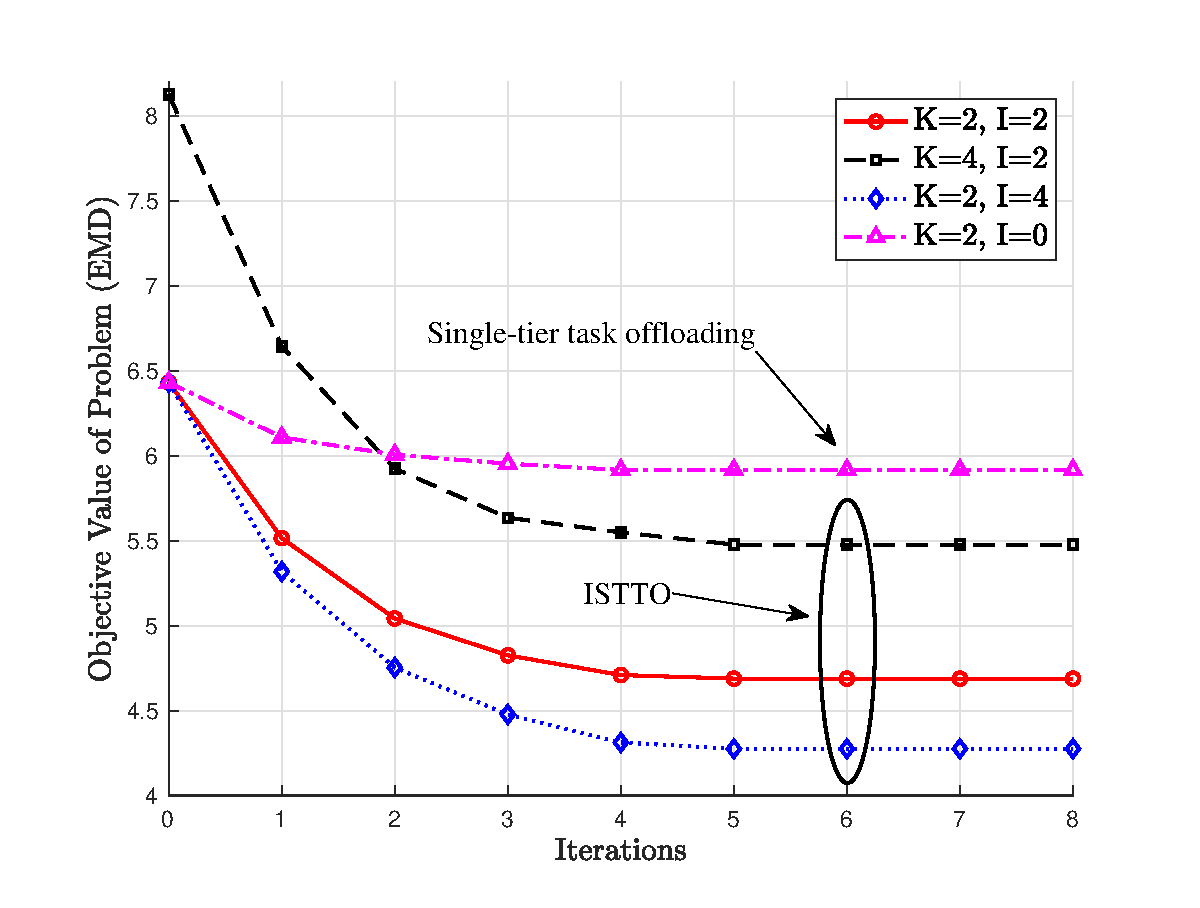
\includegraphics[width=0.6\textwidth]{figs_twc2_cld/Figure2.eps}
	\caption{Convergence performance of the proposed Algorithm 13}
	\label{chap5fig2}
\end{figure}





Figure \ref{chap5fig2} validates the convergence performance of the proposed Algorithm 13 under the different ECU numbers and CS numbers. Figure \ref{chap5fig2} demonstrates that the objective value of Problem (EMD) converges rapidly within 8 iterations for all tested cases. Meanwhile, it can be observed that the total energy consumption increases with the growing number of ECUs and decreases with the growing number of CSs, which can be explained as follows. Under the same computational offloading latency constraints, the increased number of ECUs results in higher total workloads, and a larger energy consumption is required to guarantee the more stringent offloading and computing requirements. The increased number of the CSs provides more flexible offloading options for the AP, and thus alleviates the computing burden on the AP. 
		
\begin{figure}
	\centering
	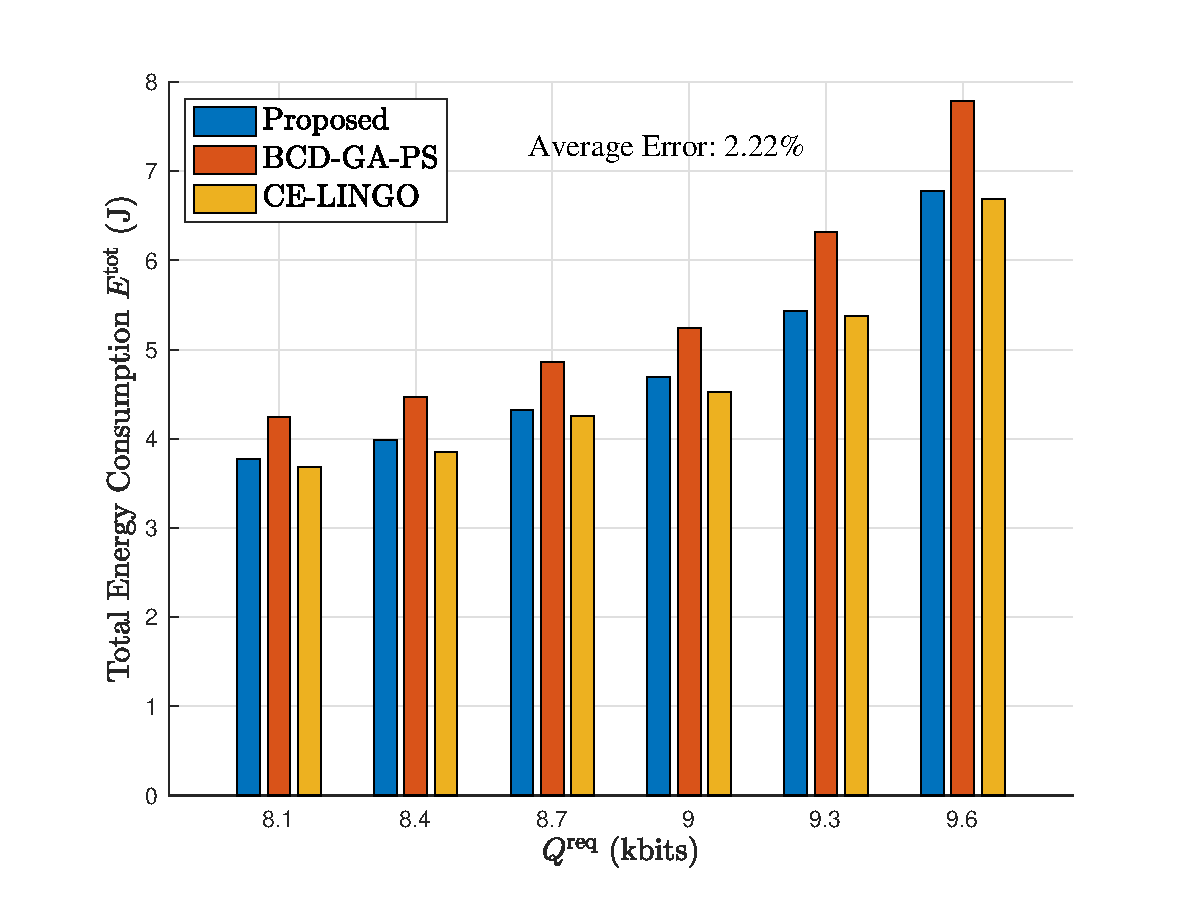
\includegraphics[width=0.6\textwidth]{figs_twc2_cld/Figure3.eps}
	\caption{Performance advantages of the proposed Algorithm 13}
	\label{chap5fig3}
\end{figure}

To verify the accuracy and effectiveness of our proposed algorithm, we compare our algorithm with the following two benchmark algorithms.
\begin{itemize}
	\item BCD-GA-PS algorithm. We utilize the BCD method to divide Problem (EMD) into two sub-problems as follows. The first sub-problem is to optimize variables $\{t^{\text{I}},t^{\text{II}}, \{d_{ki}\}\}$, which is solved by the genetic algorithm (GA) \cite{tvt.holland1992genetic}. The second sub-problem is to optimize $\{\{\mathbf{w}_i\},\mathbf{s}_0^{\text{I}},\mathbf{s}_0^{\text{II}}\}$, which is solved by the pattern search (PS) algorithm \cite{twc2.hough2001asynchronous}.
	\item CE-LINGO algorithm. We utilize the cross-entropy (CE) algorithm to find the optimal $\{t^{\text{I},\ast},t^{\text{II},\ast}, \{d_{ki}^\ast\}\}$ \cite{tvt.de2005tutorial}. For each given $\{t^{\text{I}},t^{\text{II}}, \{d_{ki}\}\}$, we obtain the solution $\{\{\mathbf{w}_i\},\mathbf{s}_0^{\text{I}},\mathbf{s}_0^{\text{II}}\}$ by LINGO \cite{twc1.schrage2006optimization}. According to the criterion of CE and LINGO, the solution obtained by CE-LINGO algorithm can be regarded as the optimal solution of Problem (EMD).
\end{itemize}
Figure \ref{chap5fig3} shows the comparison between our proposed Algorithm 13 and two benchmark algorithms versus different sensing estimation information requirements. It can be observed that our Algorithm 13 outperforms the BCD-GA-PS algorithm in energy minimization while reaching the close-to-optimal solution compared to the CE-LINGO algorithm. We mark the average error between the results obtained by our Algorithm 13 and those obtained by CE-LINGO algorithm at the top of Figure \ref{chap5fig3}. The results show that the average error does not exceed 3\%, which verifies the accuracy of our algorithm.

\begin{figure}
	\centering
	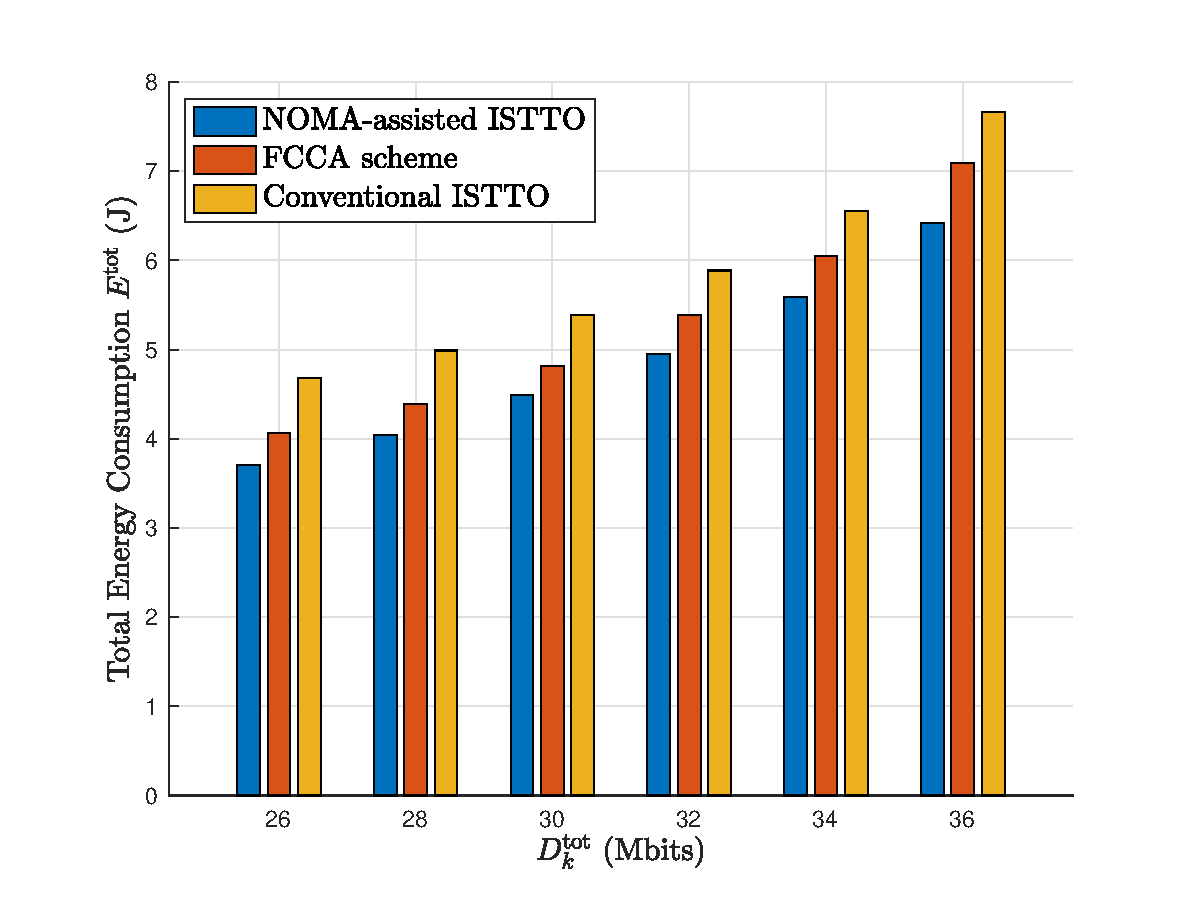
\includegraphics[width=0.6\textwidth]{figs_twc2_cld/Figure4.eps}
	\caption{Performance advantages under different $D_k^{\text{tot}}$}
	\label{chap5fig4}
\end{figure}

\begin{figure}
	\centering
	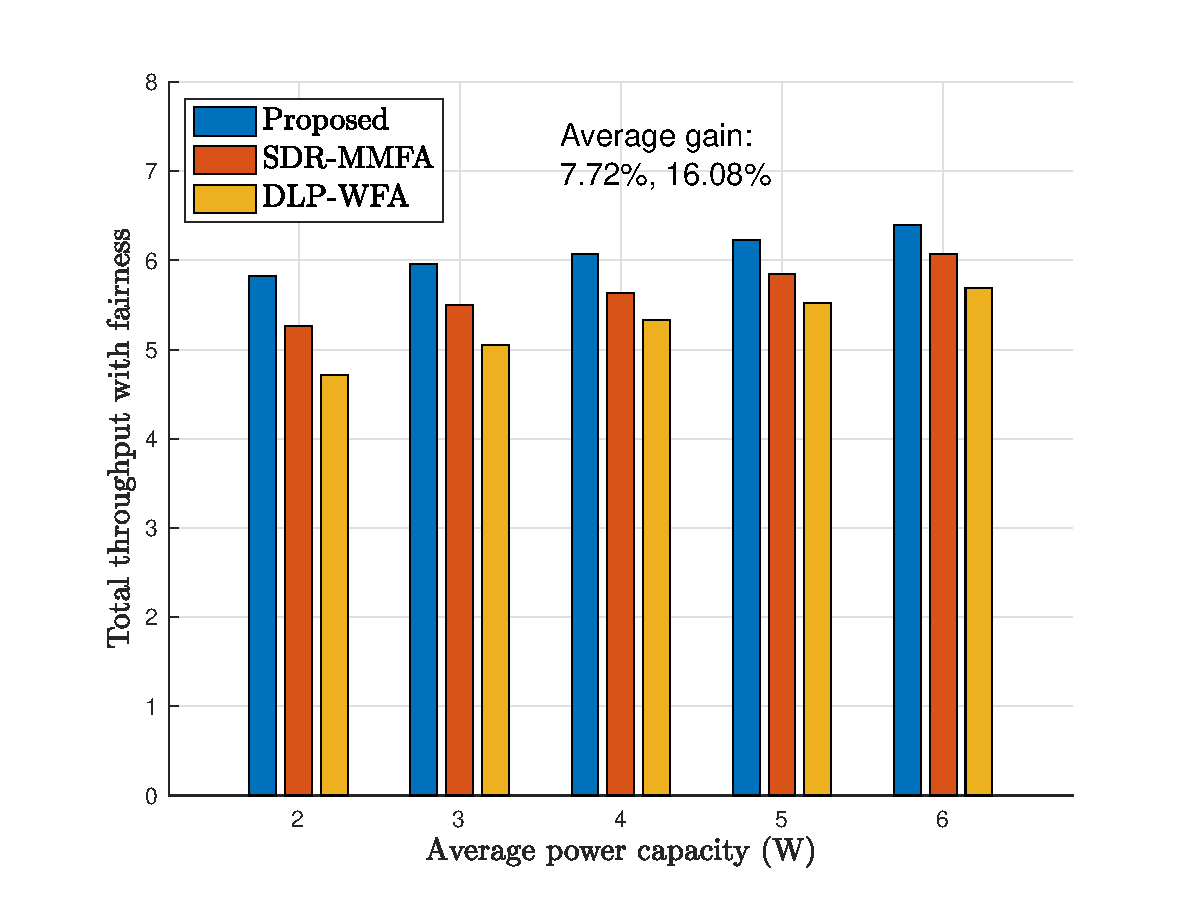
\includegraphics[width=0.6\textwidth]{figs_twc2_cld/Figure5.eps}
	\caption{Performance advantages under different $T^{\text{max}}$}
	\label{chap5fig5}
\end{figure}




Figures \ref{chap5fig4} and \ref{chap5fig5} show the performance advantages of the proposed NOMA-assisted ISTTO in comparison with two benchmark resource allocation schemes, i.e., 1) fixed computing capacity allocation (FCCA) scheme, in which the ES allocates a fixed computing capacity to each ECU and 2) conventional ISTTO, in which both tiers of transmissions do not use NOMA. Figure \ref{chap5fig4} shows that the total energy consumption is increasing with respect to the value of $D_k^{\text{tot}}$. Figure \ref{chap5fig5} shows that the total energy consumption is decreasing with respect to the value of the maximum available radio interface time $T^{\text{max}}$. It can be seen that compared to the FCCA scheme, our proposed NOMA-assisted ISTTO can achieve a lower energy consumption due to the optimized computing capacity allocation of the ES. Moreover, our NOMA-assisted ISTTO scheme significantly outperforms conventional ISTTO scheme due to the fact that leveraging NOMA alleviates the inter-functionalities interference of two-tier transmissions and thus improves both sensing and offloading performances.

\begin{figure}
	\centering
	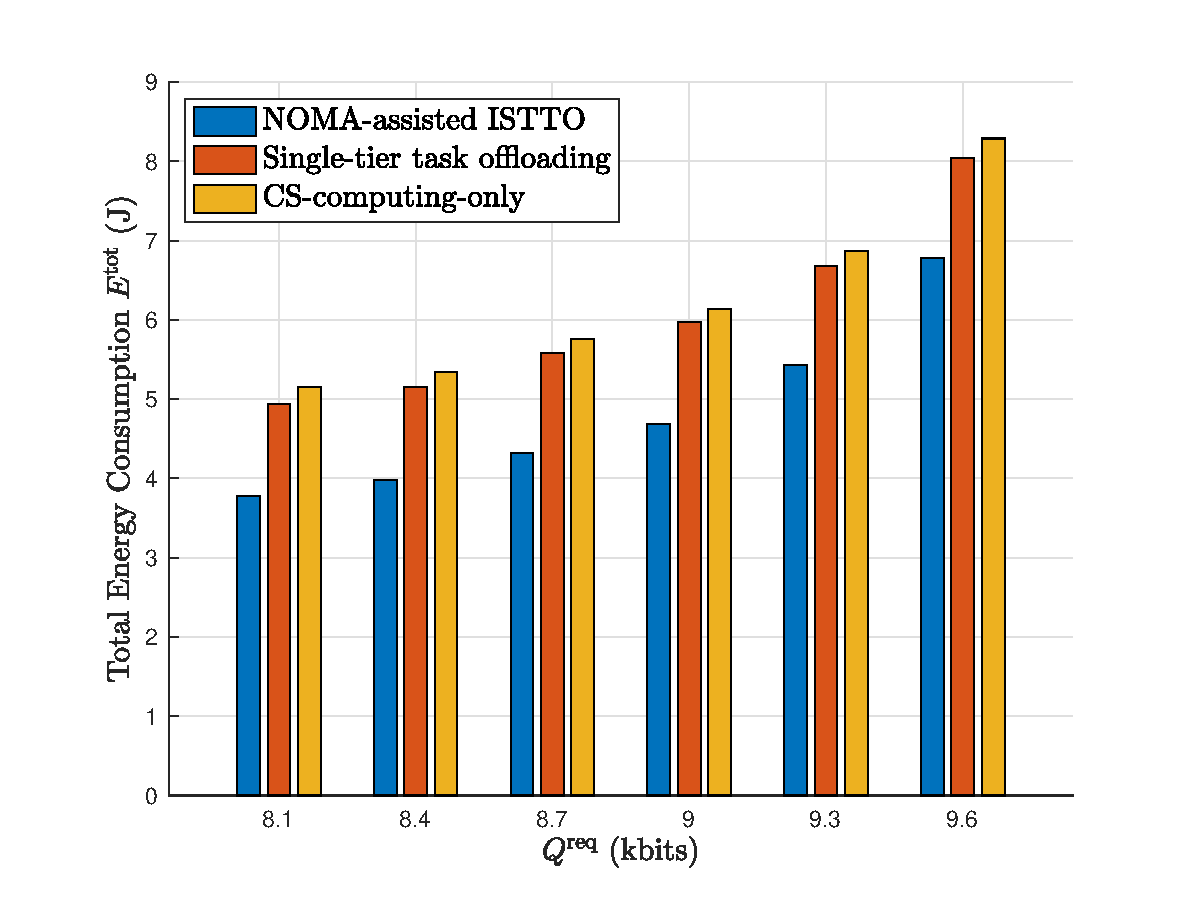
\includegraphics[width=0.6\textwidth]{figs_twc2_cld/Figure6.eps}
	\caption{Performance advantages under different $Q^{\text{req}}$}
	\label{chap5fig6}
\end{figure}

\begin{figure}
	\centering
	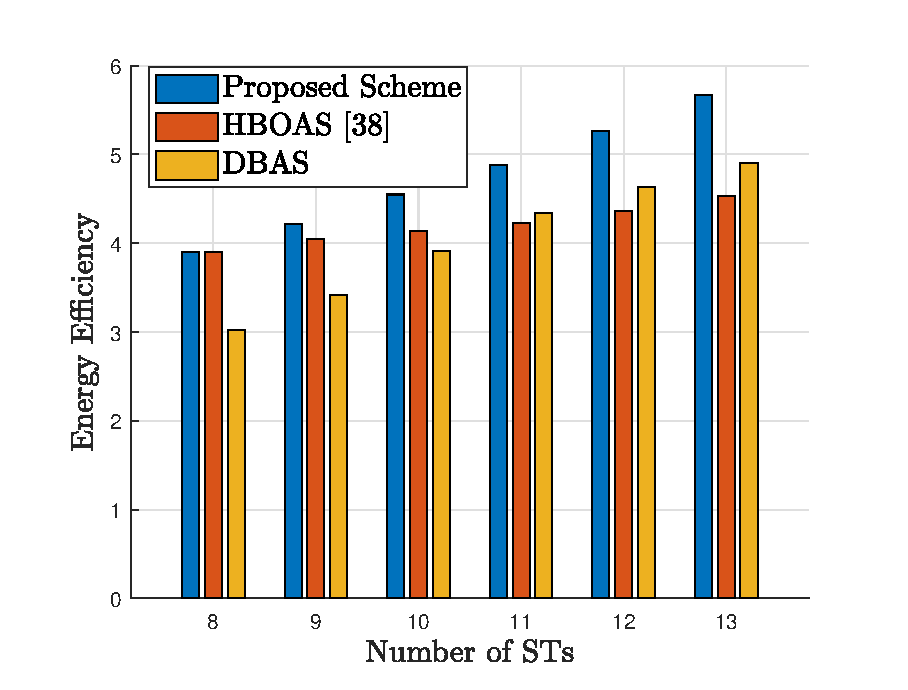
\includegraphics[width=0.6\textwidth]{figs_twc2_cld/Figure7.eps}
	\caption{Performance advantages under different $L_k^{\text{max}}$}
	\label{chap5fig7}
\end{figure}



Figures \ref{chap5fig6} and \ref{chap5fig7} demonstrate the performance advantages of our NOMA-assisted ISTTO in comparison with two benchmark offloading schemes including the single-tier task offloading scheme and the CS-computing-only scheme (all ECUs' workloads are only processed at the CSs). It can be observed that our NOMA-assisted ISTTO outperforms two benchmark offloading schemes, which indicates that our ISTTO framework can achieve a lower energy consumption than the benchmark schemes under the same computational offloading latency constraints and the sensing requirement. This is due to the fact that the two-tier task offloading framework enables an efficient and balanced utilization of the computing resources across different tiers.

\begin{figure}
	\centering
	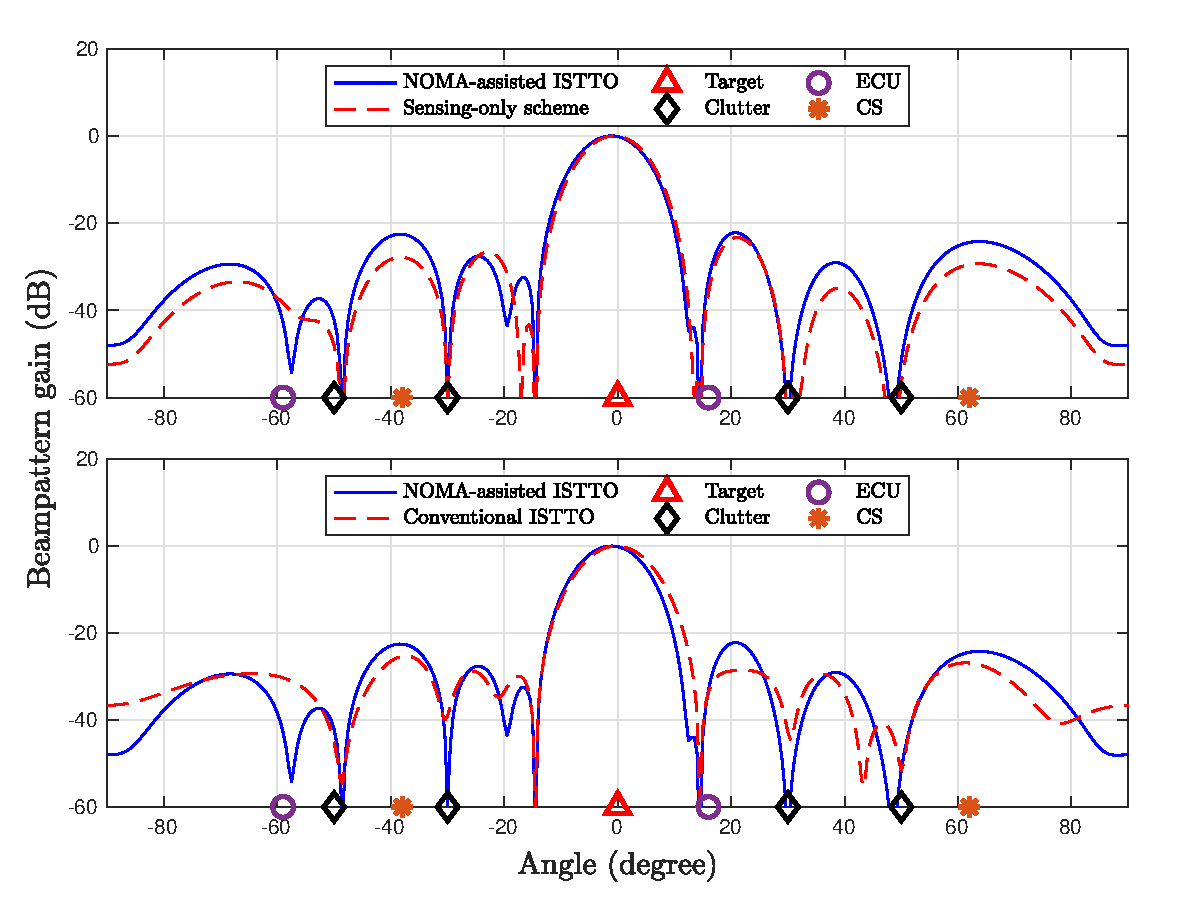
\includegraphics[width=0.6\textwidth]{figs_twc2_cld/Figure8.eps}
	\caption{Beampattern gain of NOMA-assisted ISTTO scheme}
	\label{chap5fig8}
\end{figure}
		

Figure \ref{chap5fig8} shows the beampattern gain of our NOMA-assisted ISTTO scheme, which can be defined as
\begin{equation}
	P^{\text{BG}}(\theta)=|(\mathbf{u}^\ast)^H\mathbf{a}_r(\theta)\mathbf{a}_t^H(\theta)\mathbf{x}_0^{\text{II},\ast}|^2,
\end{equation}
where the optimal sensing receiver is normalized as $||\mathbf{u}^\ast||=1$. We set $K=2$ ECUs and $I=2$ CSs as the tested scenario, and we mark the angles of all ECUs, CSs, target and clutters in both sub-figures of Figure \ref{chap5fig8}. In the top sub-figure of Figure \ref{chap5fig8}, we compare the beampattern gain achieved by our NOMA-assisted ISTTO scheme and the sensing-only scheme. It can be observed that our NOMA-assisted ISTTO scheme achieves dominant peaks in the directions of the CSs and the target, while maintaining a low power leakage in the directions of the ECUs and the clutters, which reduces the severe interference caused by reflected signals to the sensing. Compared to the sensing-only scheme, our scheme achieves higher powers in the directions of the CSs, which results in an improved two-tier task offloading performance. The bottom sub-figure of Figure \ref{chap5fig8} shows that compared to conventional ISTTO scheme, our NOMA-assisted ISTTO scheme suppresses the interference from the clutters' and the ECUs' directions better, and thus achieves a better sensing performance while maintaining the power in the directions of the CSs.


\section{Conclusion}\label{chap5_sec_conclution}
In this chapter, we have proposed a NOMA-assisted integrated sensing and two-tier task offloading system, in which the ISCC AP provides task offloading services for the ECUs while performing sensing towards a target. We have proposed a joint optimization of the AP's transmit beamforming, the two-tier dedicated sensing signals, the two-tier computation offloading strategies and the associated allocations of the communication and computing resources, with the aim of achieving an energy-minimizing design. Despite the non-convexity of the formulated joint optimization problem, we have exploited a decomposition-based framework and proposed the corresponding algorithms for solving it. Numerical results have been provided to validate the accuracy and
effectiveness of our algorithms and the performance advantages
of our NOMA-assisted ISTTO scheme.